\documentclass[12pt]{article}

%-------------PACKAGES------------- 
\usepackage[margin=1in]{geometry} 
\usepackage{amsmath,amsthm,amssymb}
\usepackage{pgfplots}
\usepackage{float}
\usepackage{braket}
\usepackage{titling}
\usepackage{tikz}
\usepackage{mathtools}
\usepackage{listings}
\usepackage{color}
\usepackage{caption}
\usepackage{subcaption}
\usepackage{algorithm,algpseudocode}

%-------------FORMATTING-------------
\setlength{\droptitle}{-5em} 
\setlength{\parindent}{0pt}
\def\LW{\dimexpr.25\linewidth-.5em} 
 
%--------------COMMANDS--------------
\newcommand{\N}{\mathbb{N}}
\newcommand{\Z}{\mathbb{Z}}
\newcommand{\R}{\mathbb{R}}
\newcommand{\C}{\mathbb{C}}
%\renewcommand{\qedsymbol}{\filledbox}

\DeclarePairedDelimiter \abs{\lvert}{\rvert}%
\DeclarePairedDelimiter \norm{\lVert}{\rVert}%

%------------ENVIRONMENTS------------- 
\newenvironment{theorem}[2][]{\begin{trivlist}
\item[{\bfseries #1}\hskip \labelsep {\bfseries #2.}]}{\end{trivlist}}
\newenvironment{lemma}[2][Lemma]{\begin{trivlist}
\item[\hskip \labelsep {\bfseries #1}\hskip \labelsep {\bfseries #2.}]}{\end{trivlist}}
\newenvironment{exercise}[2][Exercise]{\begin{trivlist}
\item[\hskip \labelsep {\bfseries #1}\hskip \labelsep {\bfseries #2.}]}{\end{trivlist}}
\newenvironment{reflection}[2][Reflection]{\begin{trivlist}
\item[\hskip \labelsep {\bfseries #1}\hskip \labelsep {\bfseries #2.}]}{\end{trivlist}}
\newenvironment{proposition}[2][Proposition]{\begin{trivlist}
\item[\hskip \labelsep {\bfseries #1}\hskip \labelsep {\bfseries #2.}]}{\end{trivlist}}
\newenvironment{corollary}[2][Corollary]{\begin{trivlist}
\item[\hskip \labelsep {\bfseries #1}\hskip \labelsep {\bfseries #2.}]}{\end{trivlist}}
\theoremstyle{remark}
\newtheorem*{remark}{Remark}

%-------------CODE-STYLE------------
\definecolor{dkgreen}{rgb}{0,0.6,0}
\definecolor{gray}{rgb}{0.5,0.5,0.5}
\definecolor{mauve}{rgb}{0.58,0,0.82}
\lstset{frame=tb,
	language=C++,
	aboveskip=3mm,
	belowskip=3mm,
	showstringspaces=false,
	columns=flexible,
	basicstyle={\small\ttfamily},
	numbers=none,
	numberstyle=\tiny\color{gray},
	keywordstyle=\color{blue},
	commentstyle=\color{dkgreen},
	stringstyle=\color{mauve},
	breaklines=true,
	breakatwhitespace=true,
	tabsize=3
}

\lstset{
	morekeywords={end}
}

%------------------------------------ 
%---------START-OF-DOCUMENT----------
%------------------------------------
\begin{document}
 
\title{Program 2}
\author{David Miller \\ 
MAD5403: Foundations of Computational Math I} 
 
\maketitle

\section{Executive Summary}

Polynomial interpolation is a powerful method in which computed polynomials are used to approximate functions or sets of data. In this program we utilize Newton, Bernstein, piecewise interpolating, and interpolatory cubic spline polynomials. Accuracy, error, and complexity of each is discussed in detail. 

\section{Statement of Problem} 

We investigate four interpolatory methods:
\begin{enumerate}
	\item Newton polynomial is an interpolation polynomial constructed given some mesh \\ $\{(x_0,y_0), \ldots, (x_n, y_n)\}$ that uses divided difference values for its coefficients. A Newton polynomial is of the form:
	\begin{equation}
	 \mathcal{N}(x) = \sum\limits_{j=0}^kc_j\prod\limits_{i=0}^{j-1}(x- x_i) 
	 \end{equation}
	where $c_j$ is the divided difference value $[x_0, \ldots, c_j]$ and the $x_i$'s are are mesh points.
	
	\item Bernstein polynomial are interpolating polynomials constructed given some mesh \\ $\{(x_0,y_0), \ldots, (x_n, y_n)\}$ defined on the unit interval $[0,1]$. A Bernstein polynomial is of the form
	\begin{equation}
	B_n(x) = \sum\limits_{k=0}^{n} f(\frac{k}{n}) {{n}\choose{k}} x^k(1-x)^{n-k}. 
	\end{equation}
	However we can easily generalize this for some arbitrary interval $[a,b]$ by mapping the following
	$$ x \rightarrow \frac{x - a}{b - a}, \quad f(\frac{k}{n}) \rightarrow f(\frac{k}{n}(b-a) + a) $$
	\item Piecewise polynomial is an interpolation polynomial where local polynomials are constructed on sub-intervals with the condition of continuity. More precisely we have a global interval $[a,b]$ with an interpolated global polynomial $p_{k,i}$, where $k$ denotes the degree of each polynomial and $i$ defines the subinterval defined on some sub-domain.  
	\item Cubic spline polynomials are piecewise polynomials with the added constraint on $p_{k,i}$ such that the values of their first $(k-1)$ derivatives also match at meshpoints $x_i$ for $1 \leq i \leq n-1$. There are also two degrees of freedom in the construction of cubic splines where we must choose two boundary conditions so that we may solve for them.
\end{enumerate}

These methods have their complexity and error analyzed and computed then compared to each other. 

\section{Description of Mathematics}

\subsection{Newton Method}

The Newton interpolating polynomial is constructed via (1). Expanding out this out we get 
\begin{align*}
	\mathcal{N}(x) = [y_0] + [y_0,y_1](x-x_0) + \ldots + [y_0,\ldots,y_k](x-x_0)(x-x_1)\ldots(x-x_{k-1}).
\end{align*}
If we investigate the form above, we can see Newton's method creates a Taylor polynomial based on the finite differences we compute, whereas Taylor's uses exact derivative values. Therefore we can view Newton's method as constructing a finite difference version of a Taylor series. Therefore as $k \rightarrow \infty$ we get that $\mathcal{N}(x)$ tends to the Taylor series. However Newton polynomials experience Runge phenomena around the boundaries since it is a single global interpolating polynomial. This is one thing piecewise fixes.

\subsection{Bernstein Method}

Bernstein polynomials provide numerically stable approximations to functions on the unit interval. In fact in can be shown that 
\begin{align*}
	\lim_{n \rightarrow \infty}(f) = f
\end{align*}
on the interval [0,1] for some function $f$. The proof will be omitted for the sake of brevity. In fact it is uniformly convergent which implies
\begin{align*}
			\lim_{n \rightarrow \infty} \sup \{\vert f(x) - B_n(f)(x) \vert: 0 \leq x \leq 1\} = 0.
\end{align*}
This is of importance because this can be used to prove the Weierstrass approximation theorem which is a pivotal theorem to us in this class.

\subsection{Piecewise Method}
Given a global interval $[a,b]$ with mesh points $a = x_0 < x_1 < \ldots < x_n = b$, we can split this up into subintervals and apply Newton's method to those subintervals and enforcing the condition of continuity and boundary points. Therefore the problem can be described with the following rules 
\begin{enumerate}
	\item $[a,b] = \cup_sI_s$ : \text{union of disjoint subintervals (intersect only at subset of mesh points)}
	\item $g_k(x),$ on $I_s = [x_{i_s}, x_{i_{s+k}}]$ is in $\mathbb{P}_k$, where $g_k(x)$ is a piecewise polynomial
	\item local interpolant $p_{k,i}(x_j) = f(x_j, \quad i_s \leq j \leq i_s + k)$
	\item global interpolant $g_k(x_i) = f(x_i), \quad 0 \leq i \leq n$
\end{enumerate}

From all this we form $p_{k,i}(x)$ where each is independent in construction and evaluation for all $i$. 

\subsection{Cubic Spline}

\subsubsection{Natural Boundary Condition}
Given our form of cubic spline we must solve

$$
\begin{pmatrix}
\mu_1 & 2 & \lambda_1 & 0 & 0 &\ldots &  \\
0 & \mu_2 & 2 & \lambda_2 & 0 & \ldots \\
& & \ddots & \ddots & \ddots & \\
0 & \ldots & & \mu_{n-1} & 2 & \lambda_{n-1}
\end{pmatrix}
\begin{pmatrix}
s^{\prime\prime}_0 \\
s^{\prime\prime}_1 \\ 
\vdots \\
s^{\prime\prime}_n
\end{pmatrix}
=
\begin{pmatrix}
d_1 \\
d_2 \\
\vdots \\
d_{n-1}
\end{pmatrix}
$$ \\

to form $p_{k,i}$. However if we are given natural boundary conditions we have that 
\begin{align*}
	s^{\prime\prime}_0 = s^{\prime\prime}_n = 0
\end{align*}
and we can rewrite the linear system as 
$$ 
\begin{pmatrix}
2 & \lambda_1 & 0 & \ldots & 0 \\
\mu_2 & 2 & \lambda_2 & 0 & \ldots \\
\ddots & \ddots & \ddots & & \\
0 &\ldots & & \mu_{n-1} & 2 
\end{pmatrix} 
\begin{pmatrix}
 s^{\prime\prime}_1 \\
 s^{\prime\prime}_2 \\
 \vdots \\
 s^{\prime\prime}_{n-1}
\end{pmatrix} 
=
\begin{pmatrix}
d_1 \\
d_2 \\
\vdots \\
d_{n-1}
\end{pmatrix}
$$ \\ 
This becomes trivial to solve using $\texttt{solveTridig()}$ then computing $p_{k,i}$ using the results from solving the linear system. 


\subsubsection{Second Hermite Boundary Condition}

Consider the second hermite boundary conditions $f^{\prime\prime}(a) = s^{\prime\prime}_0$ and $f^{\prime\prime}(b) = s^{\prime\prime}_n$ on our global interval $[a,b]$. Taking this into account we can rewrite the system 

With substitution we get the two equations
\begin{align*}
d_1 - \mu_1f^{\prime\prime}(a) & = 2s^{\prime\prime}_1 + \lambda_1s^{\prime\prime}_2 \\
d_{n-1} - \lambda_{n-1}f^{\prime\prime}(b) & = \mu_{n-1}s^{\prime\prime}_{n-2} + 2s^{\prime\prime}_{n-1}
\end{align*}

This allows us to have a square matrix which we can pass into the $\texttt{solveTridig()}$ and we just have to do four simple overwrites to our data
\begin{align*}
\text{Update array element: } & s^{\prime\prime}_0 \leftarrow f^{\prime\prime}(a) \\
\text{Update array element: } & s^{\prime\prime}_{n} \leftarrow f^{\prime\prime}(b) \\
\text{Update array element: } & d_1 \leftarrow d_1 - \mu_1f^{\prime\prime}(a) \\
\text{Update array element: } & d_{n-1} \leftarrow d_{n-1} - \lambda_{n-1}f^{\prime\prime}(b)
\end{align*}

This gives us sufficient information to solve when given second Hermite boundary conditions. \\

\section{Description of the Algorithm and Implementation}

The Divided Difference algorithm has time complexity $\mathcal{O}(n^2)$, where $n$ is the degree, while having space complexity $\mathcal{O}(n)$ to store the values of the divided differences. This is because we have a nested for loop that iterates up to $n-1$ and stores a value every time in the nested for loop.
\\

\textbf{Input:} x-Mesh $X$, y-Mesh $Y$, results $R$, degree \\
\textbf{Output:} None, we store the results in the array passed in.
\begin{algorithm}[H]
	\caption{Divided Difference}
	\begin{algorithmic}[1]	
		\For{$i = 0:1:degree$}
		\State{$R_i] \leftarrow Y_i$}
		\EndFor
		\State{$level \leftarrow 1$}
		\For{$i=0:1:degree-1$}
		\For{$j=degree:-1:1$}
		\State{$R_j \leftarrow (R_j - R_{j-1})/(X_j - X_{j-level})$}
		\EndFor
		\State{$level \leftarrow level + 1$}
		\EndFor	 
	\end{algorithmic}
\end{algorithm}

The Newton Method algorithm has time complexity $\mathcal{O}(n^2)$, where $n$ is the degree, while having space complexity $\mathcal{O}(n)$ to store values of divided difference values when \texttt{dividedDifference()} is called and to store $m$ results, where $m$ is the amount of points we pass in to evaluate at. If we take into account all the values we are evaluating at then the time complexity of Newton method becomes $\mathcal{O}(mn^2)$.
\\ 

\textbf{Input:} points $P$, numPoints, x-Mesh $X$, y-Mesh $Y$, degree, 	results $R$ \\
\textbf{Output:} None, we store the results in the array passed in.
\begin{algorithm}[H]
\caption{Newton Method}
\begin{algorithmic}[1]	
	\State{\textbf{newtonMethod}$(xMesh, \, yMesh, \, C, \, degree)$}
	\For{$i = 0:1:numPoints$}
	\State{$value \leftarrow C_0$}
	\For{$j=1:1:degree$}
	\State{$product \leftarrow 1$}
	\For{$k=0:1:j-1$}
	\State{$product \leftarrow 	prodcut(P_i - X_k)$}
	\EndFor
	\State{$value \leftarrow C_j * product$}
	\EndFor
	\State{$R_i \leftarrow value$}
	\EndFor	 
\end{algorithmic}
\end{algorithm}

The Bernstein Method algorithm has time complexity $\mathcal{O}(n)$, where $n$ is the degree, while having space complexity $\mathcal{O}(n)$ since we only have to pass yMesh values and store one temporary variable for the result value. However since the \texttt{nChooseK()} function takes linear time with respect to $n$ we have that Bernstein has time complexity $\mathcal{O}(n^2)$. However we can sacrifice some space complexity and compute all values of $\texttt{nChoosek()}$ once and store them. Then our Bernstein algorithm will have time complexity $\mathcal{O}(n)$ still with linear storage. \\

\textbf{Input: } point $p$, y-Mesh $Y$, degree, leftBound, rightBound \\
\textbf{Output: } Approximation of function we are interpolating

\begin{algorithm}[H]
	\caption{Bernstein Method}
	\begin{algorithmic}[1]	
		\State{$result \leftarrow 0$}
		\State{$x \leftarrow (p - leftBound)/(rightBound - leftBound)$}
		\For{$i=0:1:degree$}
		\State{$result \leftarrow Y_i * {{n}\choose{i}} * f^i * (1 - f)^{n-i}$}
		\EndFor \\
		\Return{result}
	\end{algorithmic}
\end{algorithm}

The Piecewise Method algorithm has time complexity $\mathcal{O}(nlogn) + \mathcal{O}(n) + \mathcal{O}(d^2)$ = $\mathcal{O}(nlogn)$, where $n$ is number of mesh points and $d$ is the degree of the interpolating polynomials. The first bound is from heap sort and the third comes from calling \texttt{newtonMethod()} with mesh size $d$. The third is not so obvious, but it comes from searching for the appropriate sub-interval and constructing it. When we search for the appropriate sub-interval we are iterating over the mesh points but with jump size $d$ since we want to jump to the next sub-interval, and then building it requires $\mathcal{O}(d)$ time, and therefore $\mathcal{O}(\frac{n}{d} * d) = \mathcal{O}(n)$. However since we evaluate at $m$ points, the complexity for this becomes $\mathcal{O}(mnlogn)$. The space complexity of Piecewise is $\mathcal{O}(n)$ since we must store results, mesh points and their values, and points to evaluate at. \\ \\
The Piecewise Method should have the mesh points sorted so that searching for the appropriate sub interval can be done. If the mesh points were not sorted then we would not be able to effectively calculate sub-intervals. To sort the mesh points, and their respective values, I implemented heap sort which is well known to be $\mathcal{O}(nlogn)$ in time and $\mathcal{O}(1)$ in memory. \\

\textbf{Input: } points $P$, numPoints, x-Mesh $X$, y-Mesh $Y$, meshSize, degree, results $R$ \\
\textbf{Output:} None, we store the results in the array passed in
\begin{algorithm}[H]
	\caption{Piecewise Method}
	\begin{algorithmic}[1]	
		\State{$subintervals \leftarrow (meshSize - 1)/degree$}
		\State{$\textbf{heapsort}(X, \, Y, \, meshSize)$}
		\For{$i=0:1:numPoints-1$}
		\For{$j=0:degree:meshSize-1$}
		\If{$P_i \geq X_j \,\, \&\& \,\, P_i \leq X_{j+degre}$}
		\For{$k=0:1:degree$}
		\State{$subX_k \leftarrow X_{j+k}$}
		\State{$subY_k \leftarrow Y_{j+k}$}
		\EndFor
		\State{$\textbf{break}$}
		\EndIf
		\EndFor
		\State{$\textbf{newtonMethod}(P_i, 1, subX, subY, degree, value)$}
		\State{$R_i \leftarrow value$}
		\EndFor
	\end{algorithmic}
\end{algorithm}

The Solve Tridiagonal algorithm, sometimes called Thomson's algorithm, has time complexity $\mathcal{O}(n)$, where $n$ is one less than the mesh size, and storage complexity $\mathcal{O}(n)$ since we have to store $n$ results. \\

\textbf{Input: } vector $a$, vector $b$, vector $c$, vector $d$, results $R$, degree \\
\textbf{Output: } \textbf{Output:} None, we store the results in the array $R$
\begin{algorithm}[H]
	\caption{Solve Tridiagonal}
	\begin{algorithmic}[1]	
		\State{$n \leftarrow meshSize - 1$}
		\For{$i=2:1:n-2$}
		\State{$c_i \leftarrow c_i/(b_i - a_i*c_{i-1})$}
		\EndFor
		\For{$i=2:1:n-1$}
		\State{$d_i \leftarrow (d_i - a_i*d_{i-1})/(b_i - a_i*c_{i-1})$}
		\EndFor
		\State{$R{n-1} \leftarrow d_{n-1}$}
		\For{$i=n-2:-1:1$}
		\State{$R_i \leftarrow d_i - c_i * R_{i+1}$}
		\EndFor
	\end{algorithmic}
\end{algorithm}

Just like the Piecewise Method, we are bounded above by the time complexity of our sorting algorithm. The time complexity of Cubic spline is $\mathcal{O}(nlogn)$ and taking into account evaluating at $m$ points the time complexity becomes $\mathcal{O}(mnlogn)$. We have $\mu, \lambda, d, M, \gamma,\tilde{\gamma}, $ and results array that store values in $\mathcal{O}(n)$ and therefore Cubic spline has $\mathcal{O}(n)$ storage complexity. \\

\textbf{Input: } points $P$, numPoints, x-Mesh $X$, y-Mesh $Y$, meshSize, results $R$ \\
\textbf{Output: } \textbf{Output:} None, we store the results in the array passed in
\begin{algorithm}[H]
	\caption{Cubic Spline}
	\begin{algorithmic}[1]	
		\State{$n \leftarrow meshSize-1$}
		\State{$\textbf{heapsort}(X, \, Y, \, meshSize)$}
		\For{$i=1:1:n-1$}
		\State{$\mu_i \leftarrow (X_i - X_{i-1}) / (X_{i+1} - X_{i-1})$}
		\State{$\lambda_i = (X_{i+1} - X_{i}) / (X_{i+1} - X_{i-1})$} 
		\State{$d_i \leftarrow 6 * (((Y_{i+1} - Y_i) / (X_{i+1} - X_i)) - 
		((Y_i - Y_{i-1}) / (X_i - X_{i-1}))) / (X_{i+1} - X_{i-1})$)}
		\EndFor
		\If{$secondHermite$}
		\State{$M_0 \leftarrow leftSecondDerivative$}
		\State{$M_n \leftarrow rightSecondDerivative$}
		\State{$d_1 \leftarrow d_1 - \mu_1 * leftSecondDerivative$}
		\State{$d_{n-1} = d_{n-1} - \lambda_{n-1}*rightSecondDerivate$}
		\EndIf \\
		\textbf{$\textbf{solveTridig}(\mu, 2, \lambda, d, M, meshSize)$}
		\For{$i=1:1:n$}
		\State{$\gamma_{i-1} \leftarrow (Y_i - Y_{	i-1})/(X_i - X_{i-1}) - (M_i - M_{i-1}) * ((X_i - X_{i-1})/6)$}
		\State{$\tilde{\gamma}_{i-1} \leftarrow Y_{i-1} - M_{i-1}*(X_i - X_{i-1})^2/2$}
		\EndFor
		\For{$i=0:1:numPoints-1$}
		\For{$j=0:1:meshSize-2$}
		\If{$P_i \geq X_j \,\, \&\& \,\, P_i \leq X_{j+1}$}
		\State{$R_i \leftarrow M_j * (X_{j+1} - P_i)^3/(6*(X_{j+1} - X_j)) + M_{j+1} * (P_i - X_j)^3 / (6*(X_{j+1} - $}
		\State{$X_j)) + \gamma_j * (P_i - X_j) + \tilde{\gamma}_j$}
		\EndIf
		\State{\textbf{break}}
		\EndFor
		\EndFor
	\end{algorithmic}
\end{algorithm}

\pagebreak

\section{Description of the Experiment Design and Results}

For this program,all the user needs to specify is the left boundary, right boundary, function to interpolate/approximate,and what boundary conditions to impose on the cubic spline algorithm. To impose mesh size or polynomial degree restrictions, we hard code it in the main function since it is faster and easier than asking the user all of these things via command line. Further details about the code will be discussed during the live code demonstration.  \\ \\

If we look at the figures, we see many things we expect to see:
\begin{itemize}
	\item Newton's Method is exhibiting Runge's Phenomena near the boundaries whereas using the Newton Method to interpolate subintervals in Piecewise does not exhibit this.
	\item Bernstein polynomials converge to the exact solution as we increase the degree of the polynomial. This is confirmed in figure 15.
	\item Figure 14(b) depicts the conditioning of the problem. Essentially we have a smaller conditioning number when $x < 0$ so our error will not be as high when $x > 0$.
	\item All interpolatory methods (everything except Bernstein's Method) that are fed order meshed points have zero error at the mesh points. Passing in a non order set will create errors at the mesh points. However Newton's method will start to incur errors near the boundaries due to Runge's Phenomena and will incur even greater error in its derivatives.
	\item The convergence rate of Bernstein is $\sqrt{n}$, where $n$ is the amount of mesh points.
\end{itemize}

\section{Conclusions}

The interpolatory and approximation methods provide accurate results. Newton's method experiences Runge's Phenomena, Bernstein's polynomial converges to what we want as we increases the degree, Piecewise uses Newton's on subintervals which get rid of Runge's phenomena, and Cubic splines provide the best approximations that also give us differentiability. The interpolatory methods incur error on the mesh points if the mesh is not sorted when passed. Due to limited amount of time, a rigorous analysis is omitted and numerical evidence is instead presented in Section 7.

\section{Figures} 

\subsection{Hermite Boundary Conditions}

\begin{figure}[H]
	\centering
	\begin{subfigure}{.5\textwidth}
		\centering
		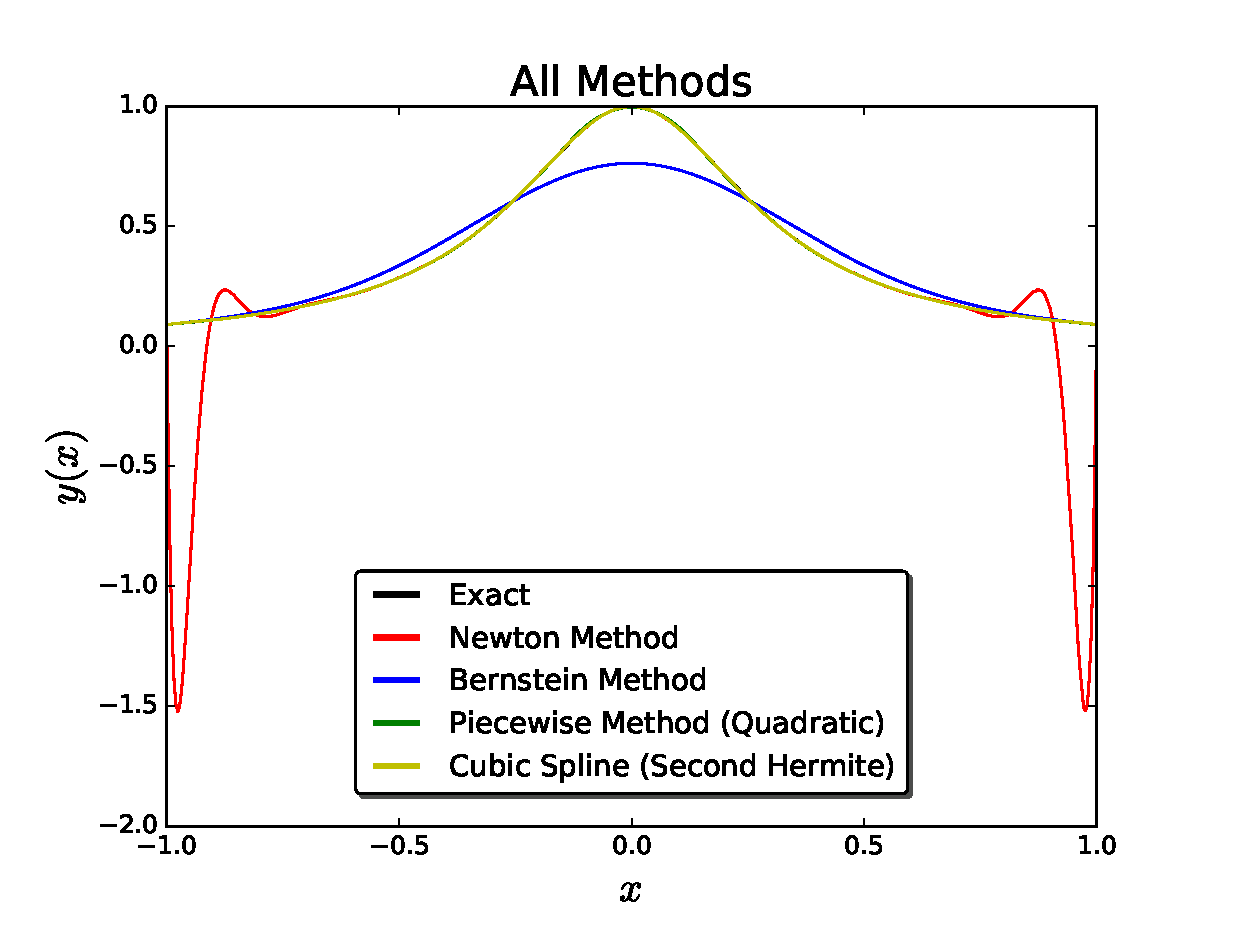
\includegraphics[width=1.1\linewidth]{fig1.eps}
		\caption{Global view of interpolating methods.}
		\label{fig:sub1}
	\end{subfigure}%
	\begin{subfigure}{.5\textwidth}
		\centering
		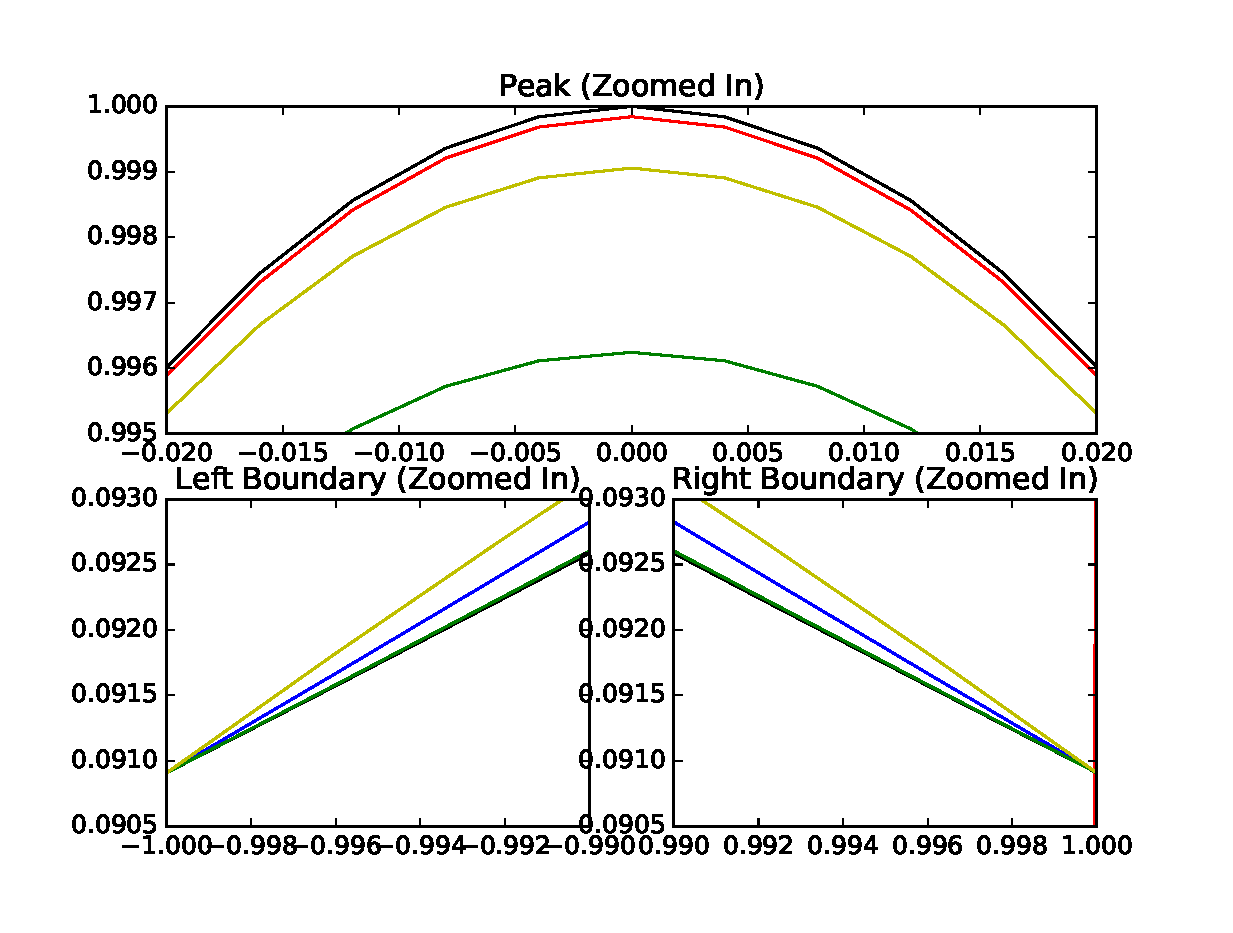
\includegraphics[width=1.1\linewidth]{subFig1.eps}
		\caption{Local view of interpolating methods.}
		\label{fig:sub2}
	\end{subfigure}
	\caption{Interpolation for $f(x) = 1/(1+10x^2)$ with 22 uniform mesh points on [-1,1].}
	\label{fig:test}
\end{figure}

\begin{figure}[H]
	\centering
	\begin{subfigure}{.5\textwidth}
		\centering
		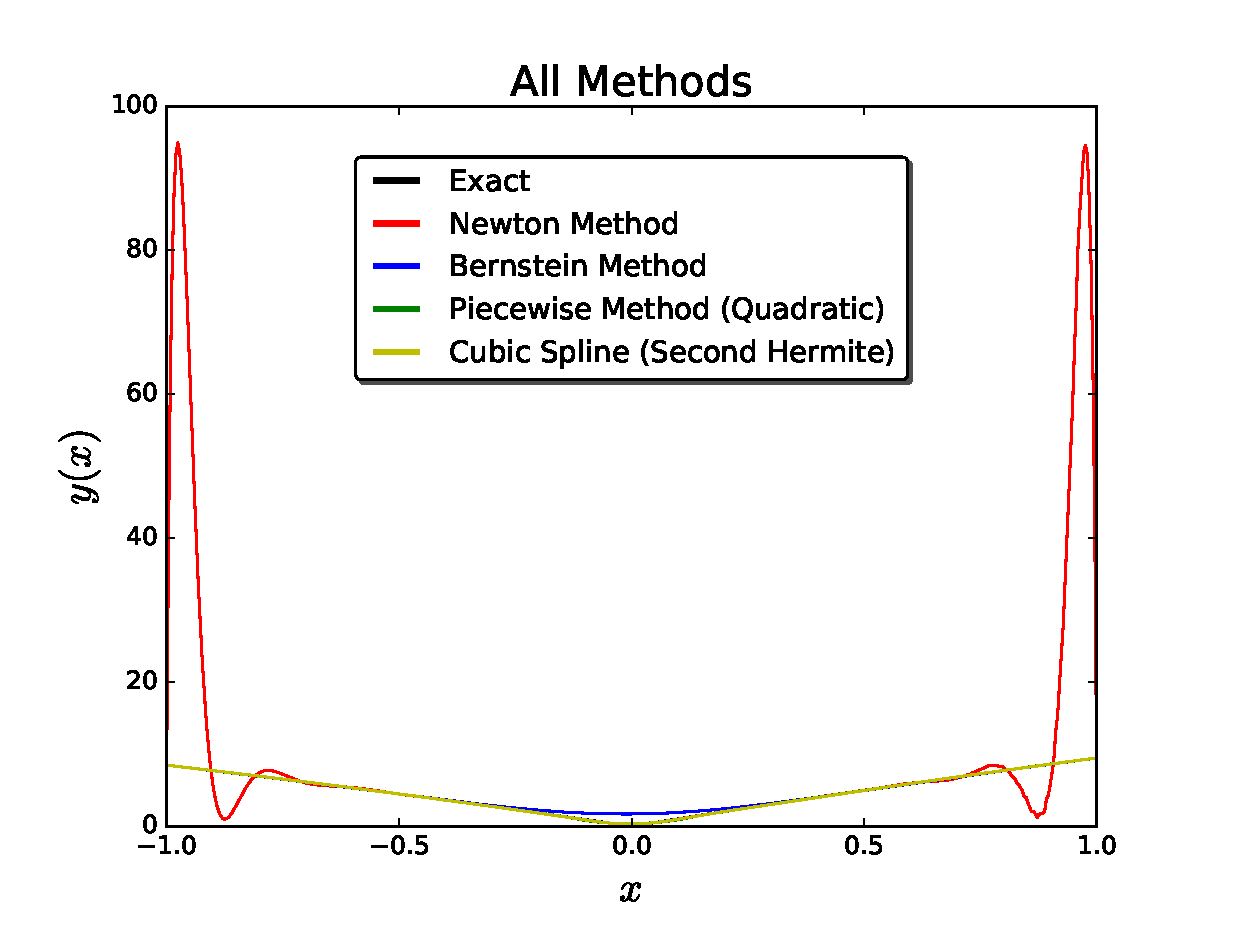
\includegraphics[width=1.1\linewidth]{fig2.eps}
		\caption{Global view of interpolating methods.}
		\label{fig:sub1}
	\end{subfigure}%
	\begin{subfigure}{.5\textwidth}
		\centering
		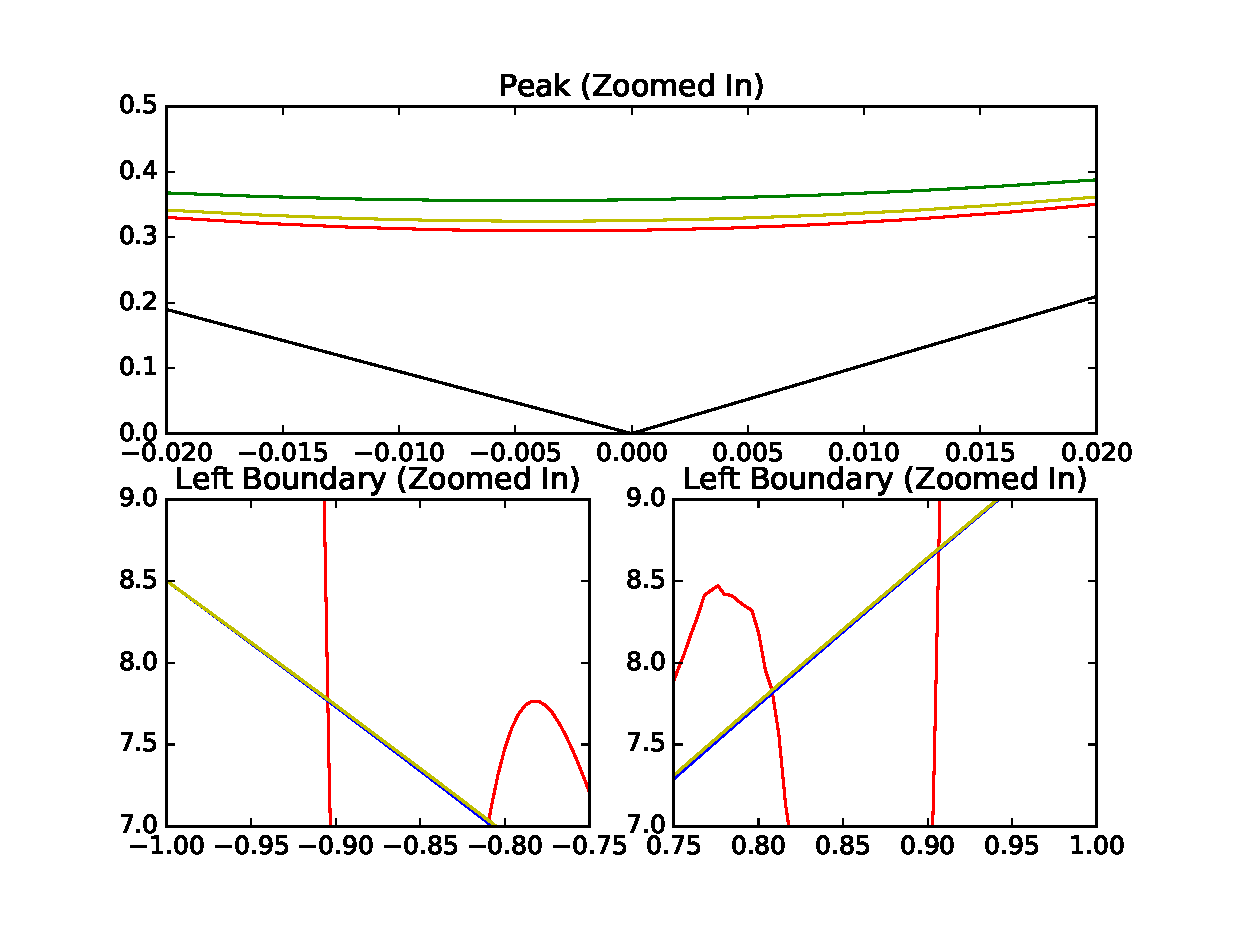
\includegraphics[width=1.1\linewidth]{subFig2.eps}
		\caption{Local view of interpolating methods.}
		\label{fig:sub2}
	\end{subfigure}
	\caption{Interpolation for $f(x) = \vert10x\vert + x/2 - x^2$ with 22 uniform mesh points on [-1,1].}
	\label{fig:test}
\end{figure}

\begin{figure}[H]
	\centering
	\begin{subfigure}{.5\textwidth}
		\centering
		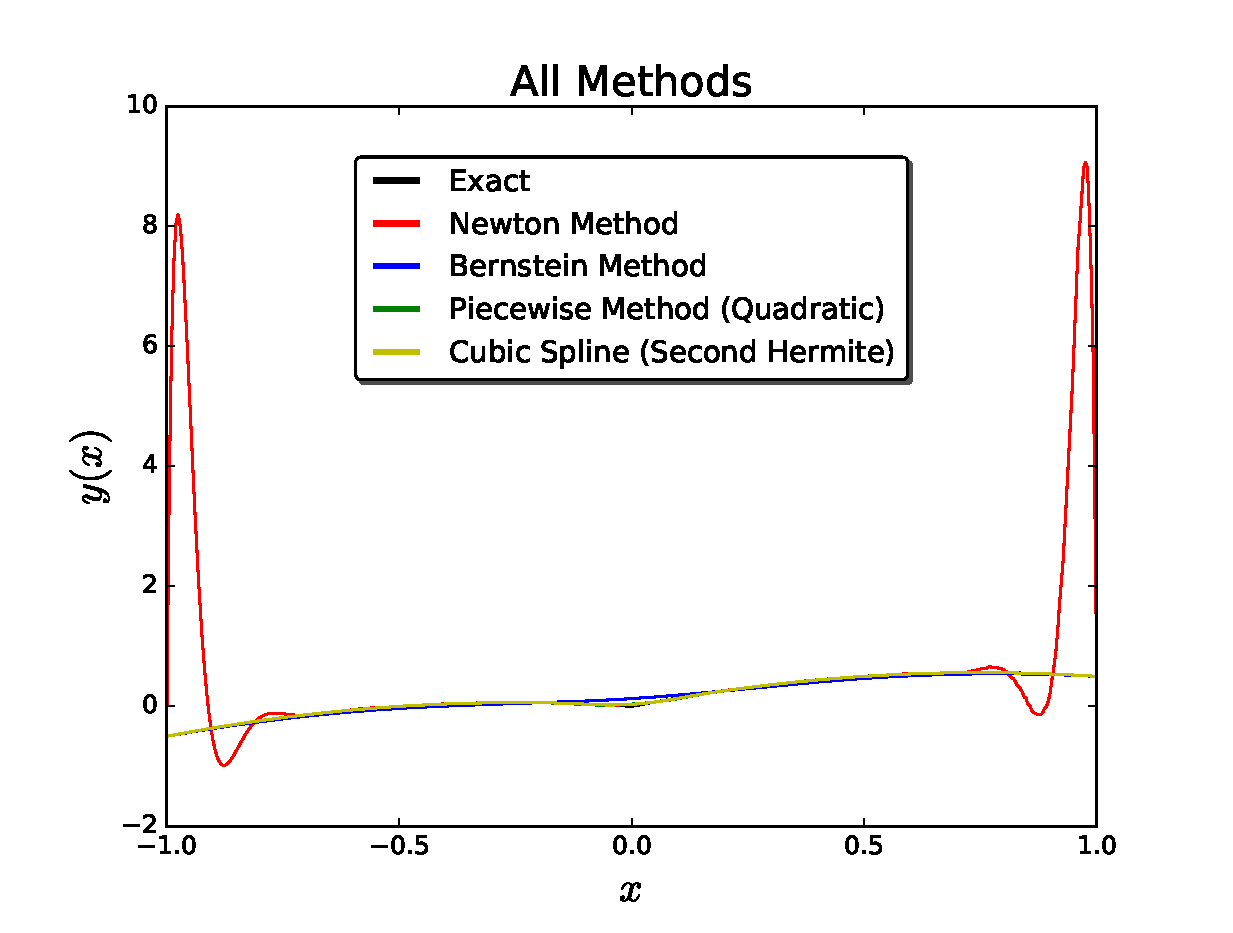
\includegraphics[width=1.1\linewidth]{fig3.eps}
		\caption{Global view of interpolating methods.}
		\label{fig:sub1}
	\end{subfigure}%
	\begin{subfigure}{.5\textwidth}
		\centering
		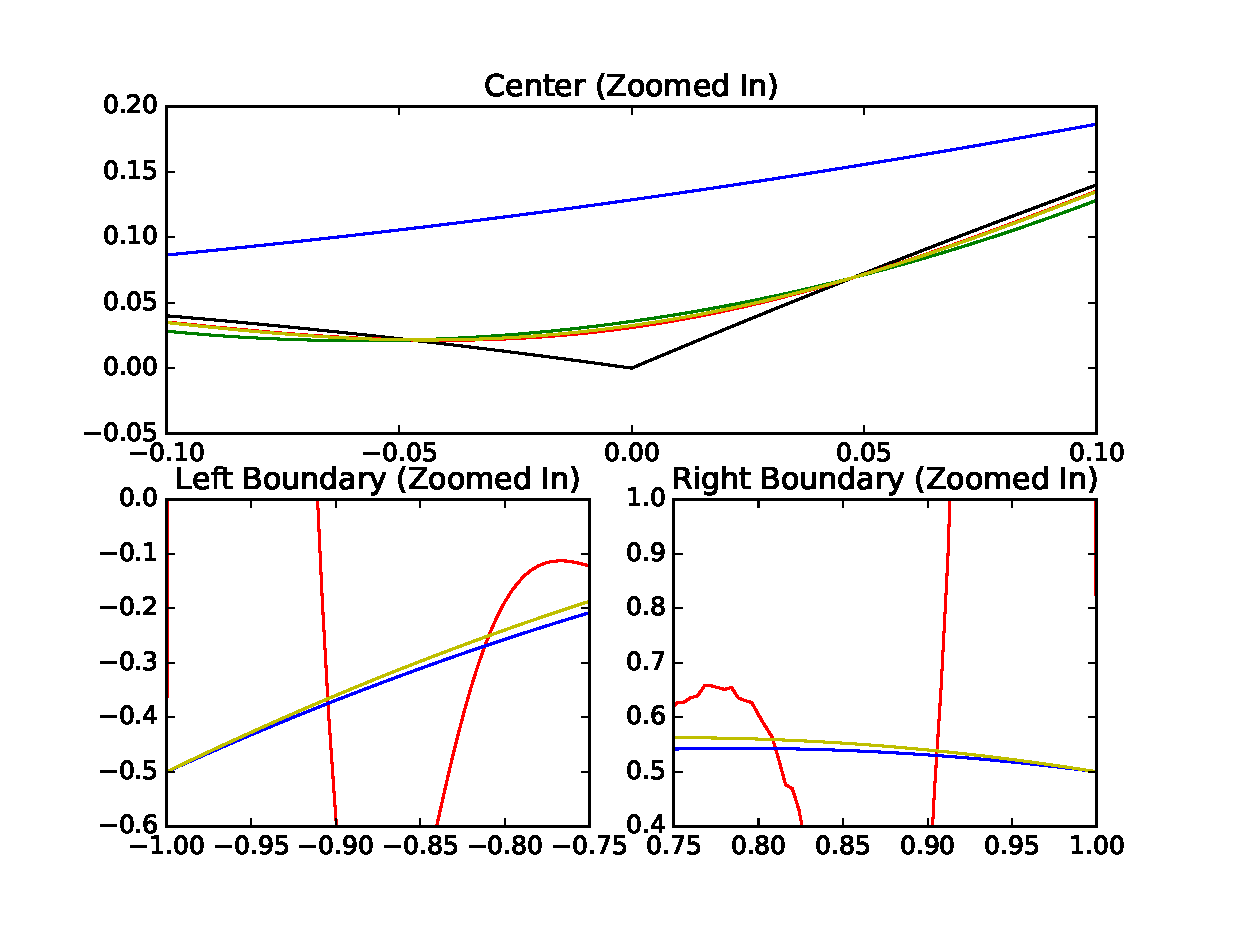
\includegraphics[width=1.1\linewidth]{subFig3.eps}
		\caption{Local view of interpolating methods.}
		\label{fig:sub2}
	\end{subfigure}
	\caption{Interpolation for $f(x) = \vert x\vert + x/2 - x^2$ with 22 uniform mesh points on [-1,1].}
	\label{fig:test}
\end{figure}

\begin{figure}[H]
	\centering
	\begin{subfigure}{.5\textwidth}
		\centering
		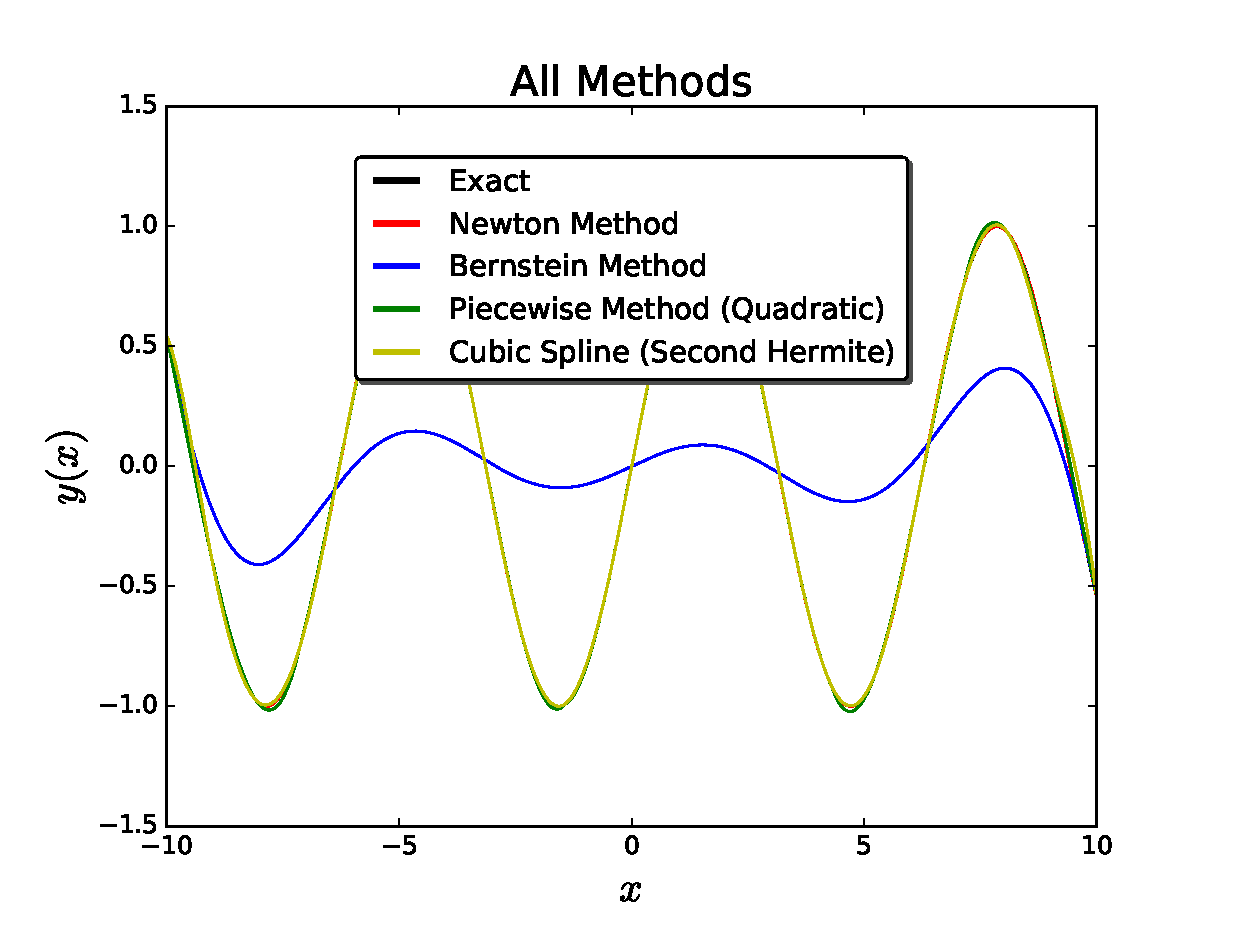
\includegraphics[width=1.1\linewidth]{fig4.eps}
		\caption{Global view of interpolating methods.}
		\label{fig:sub1}
	\end{subfigure}%
	\begin{subfigure}{.5\textwidth}
		\centering
		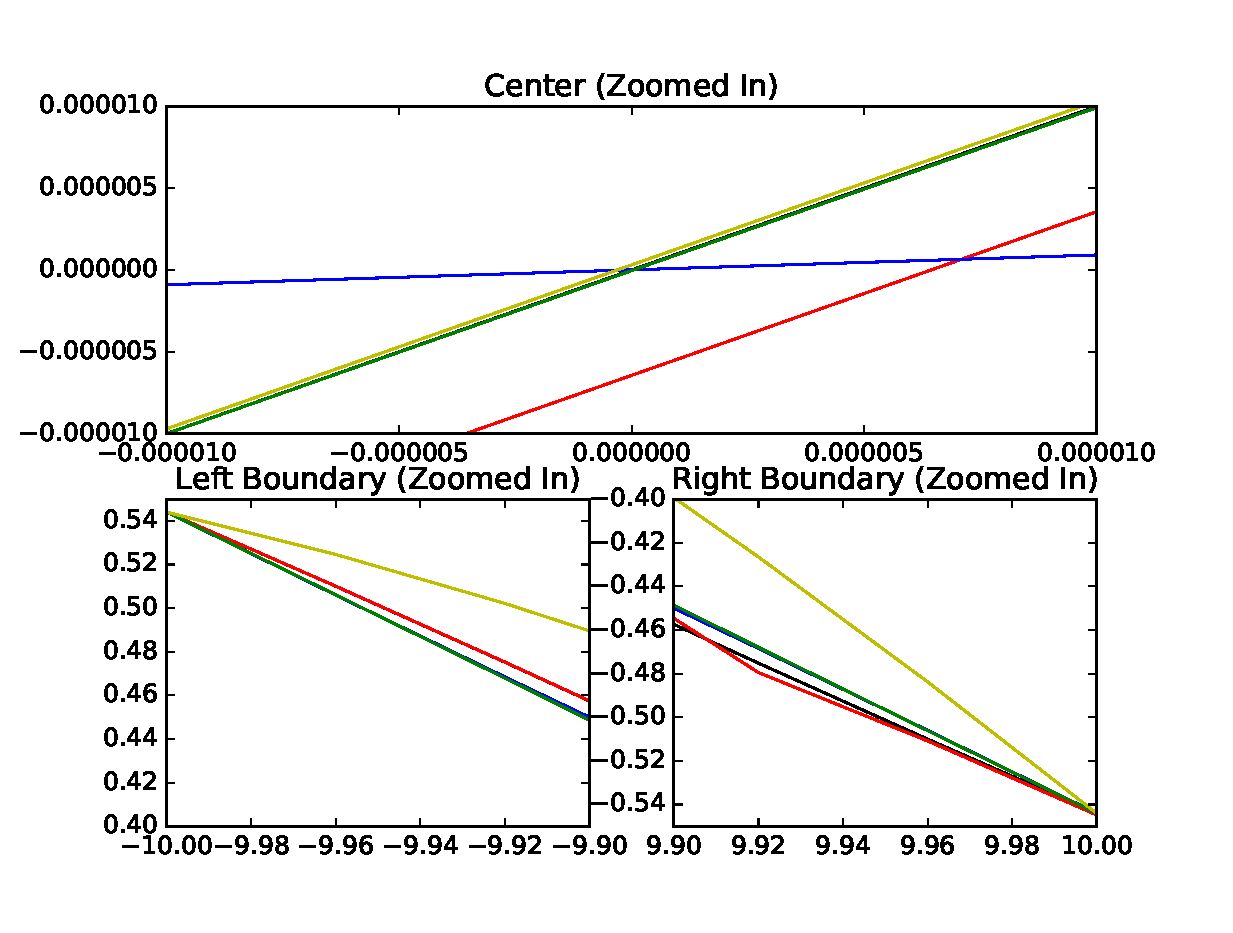
\includegraphics[width=1.1\linewidth]{subFig4.eps}
		\caption{Local view of interpolating methods.}
		\label{fig:sub2}
	\end{subfigure}
	\caption{Interpolation for $f(x) = sin(x)$ with 22 uniform mesh points on [-10,10].}
	\label{fig:test}
\end{figure}

\begin{figure}[H]
	\centering
	\begin{subfigure}{.5\textwidth}
		\centering
		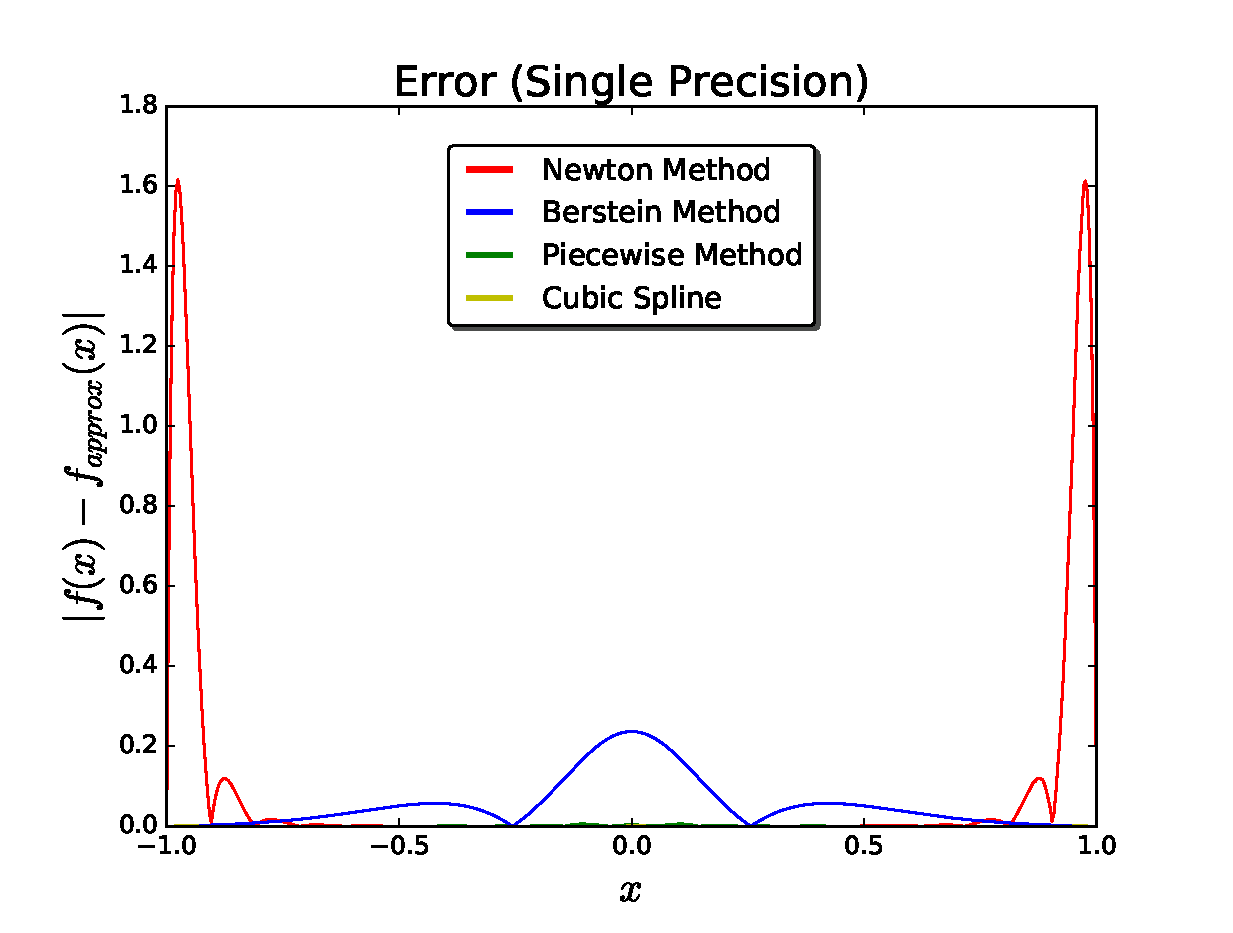
\includegraphics[width=1.1\linewidth]{errorFig1.eps}
		\caption{Global view of error.}
		\label{fig:sub1}
	\end{subfigure}%
	\begin{subfigure}{.5\textwidth}
		\centering
		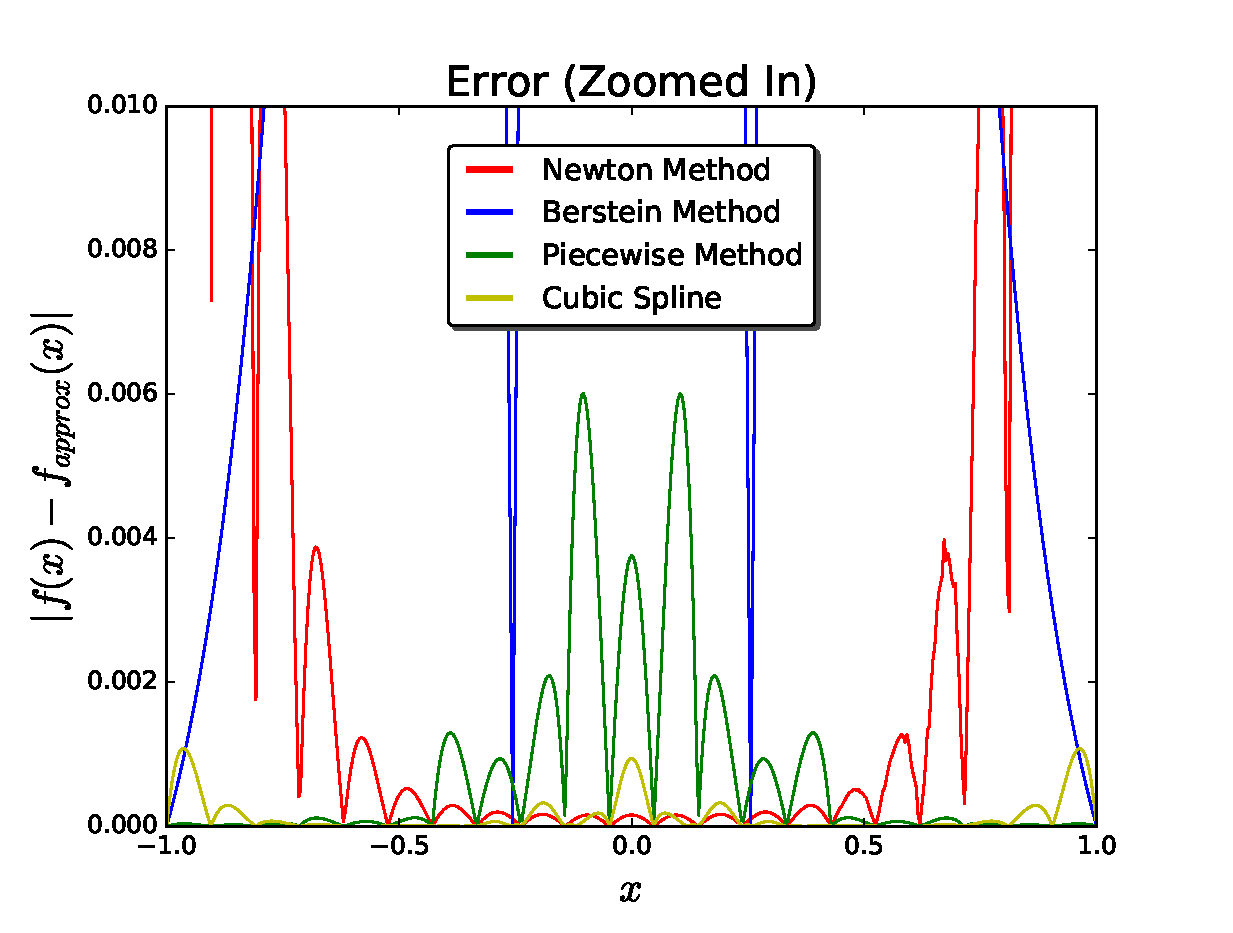
\includegraphics[width=1.1\linewidth]{errorFigg1.eps}
		\caption{Local view of error.}
		\label{fig:sub2}
	\end{subfigure}
	\caption{Error for interpolating methods $f_{approx}(x)$ vs exact $f(x) = 1/(1 + 10x^2)$ (double precision evaluation). }
	\label{fig:test}
\end{figure}

\begin{figure}[H]
	\centering
	\begin{subfigure}{.5\textwidth}
		\centering
		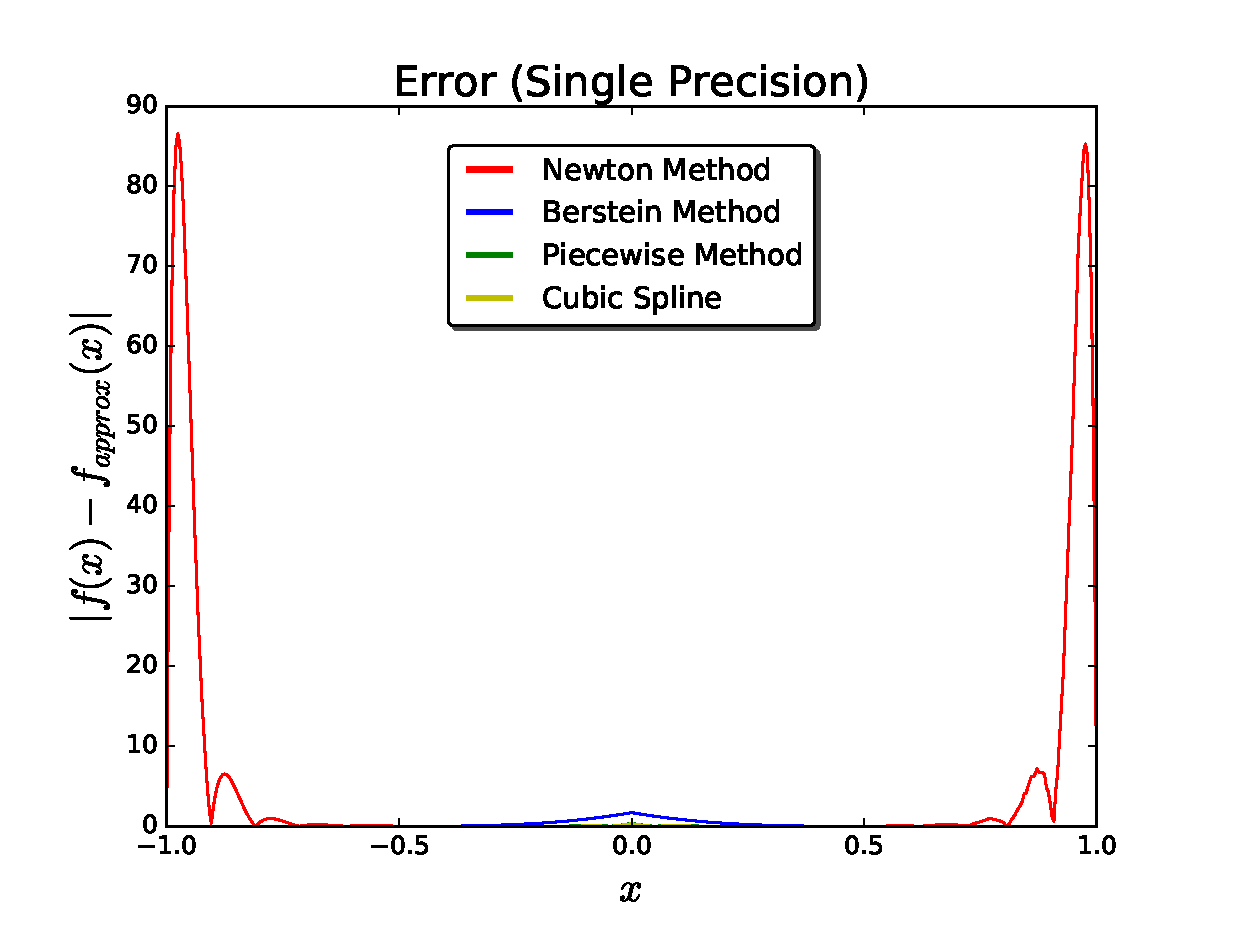
\includegraphics[width=1.1\linewidth]{errorFig2.eps}
		\caption{Global view of error.}
		\label{fig:sub1}
	\end{subfigure}%
	\begin{subfigure}{.5\textwidth}
		\centering
		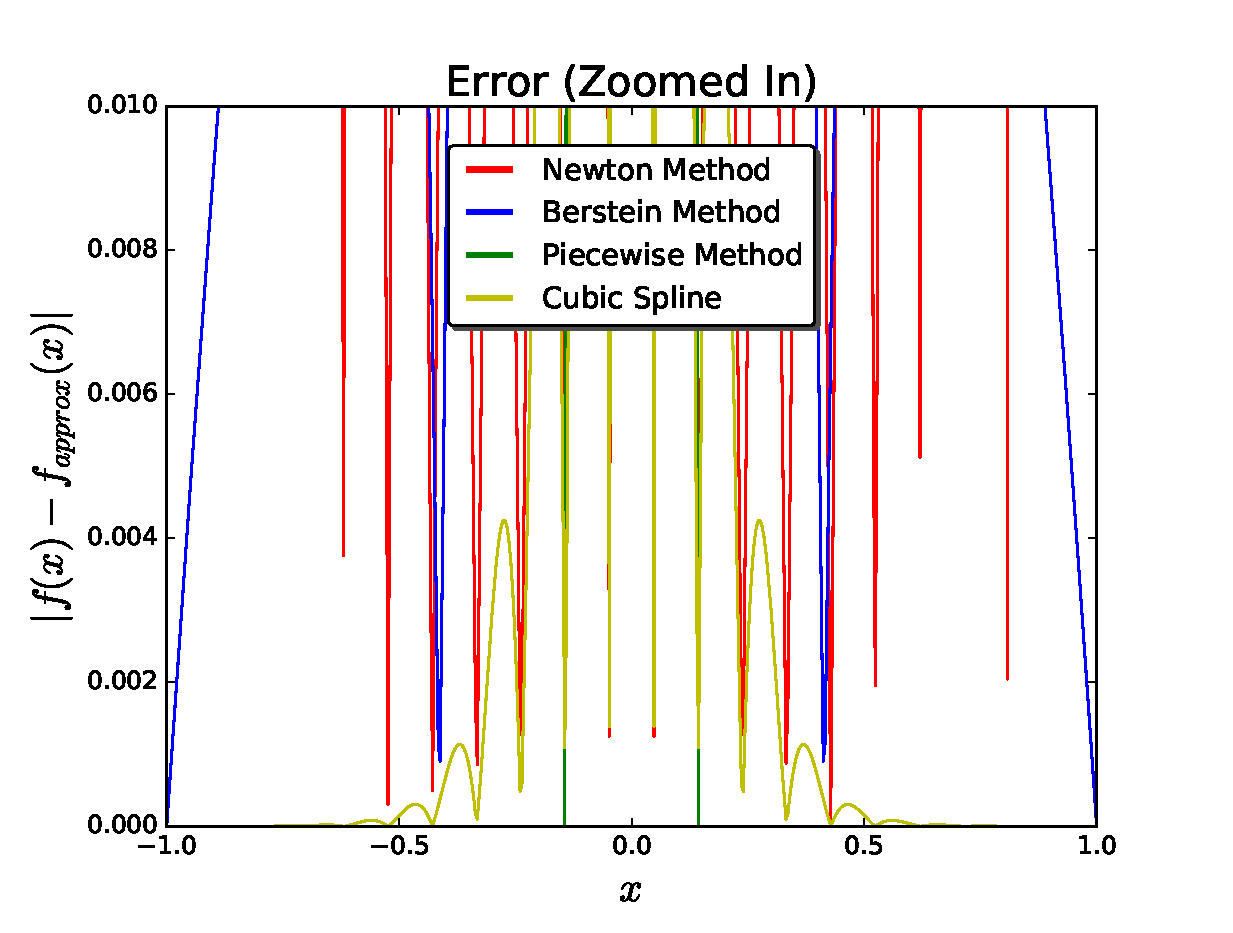
\includegraphics[width=1.1\linewidth]{errorFigg2.eps}
		\caption{Local view of error.}
		\label{fig:sub2}
	\end{subfigure}
	\caption{Error for interpolating methods $f_{approx}(x)$ vs exact $f(x) = \vert 10x \vert + x/2 - x^2$ (double precision evaluation). }
	\label{fig:test}
\end{figure}

\begin{figure}[H]
	\centering
	\begin{subfigure}{.5\textwidth}
		\centering
		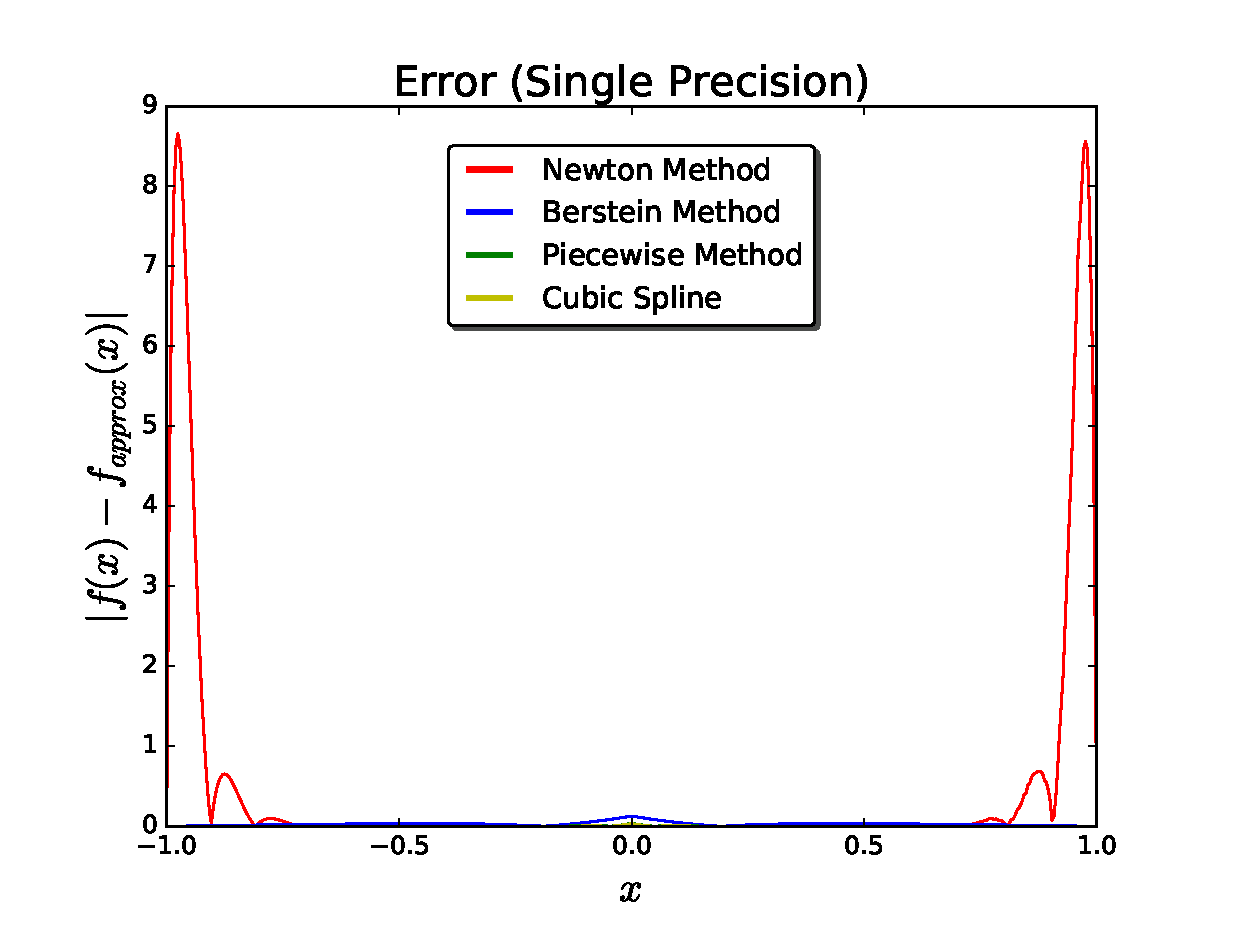
\includegraphics[width=1.1\linewidth]{errorFig3.eps}
		\caption{Global view of error.}
		\label{fig:sub1}
	\end{subfigure}%
	\begin{subfigure}{.5\textwidth}
		\centering
		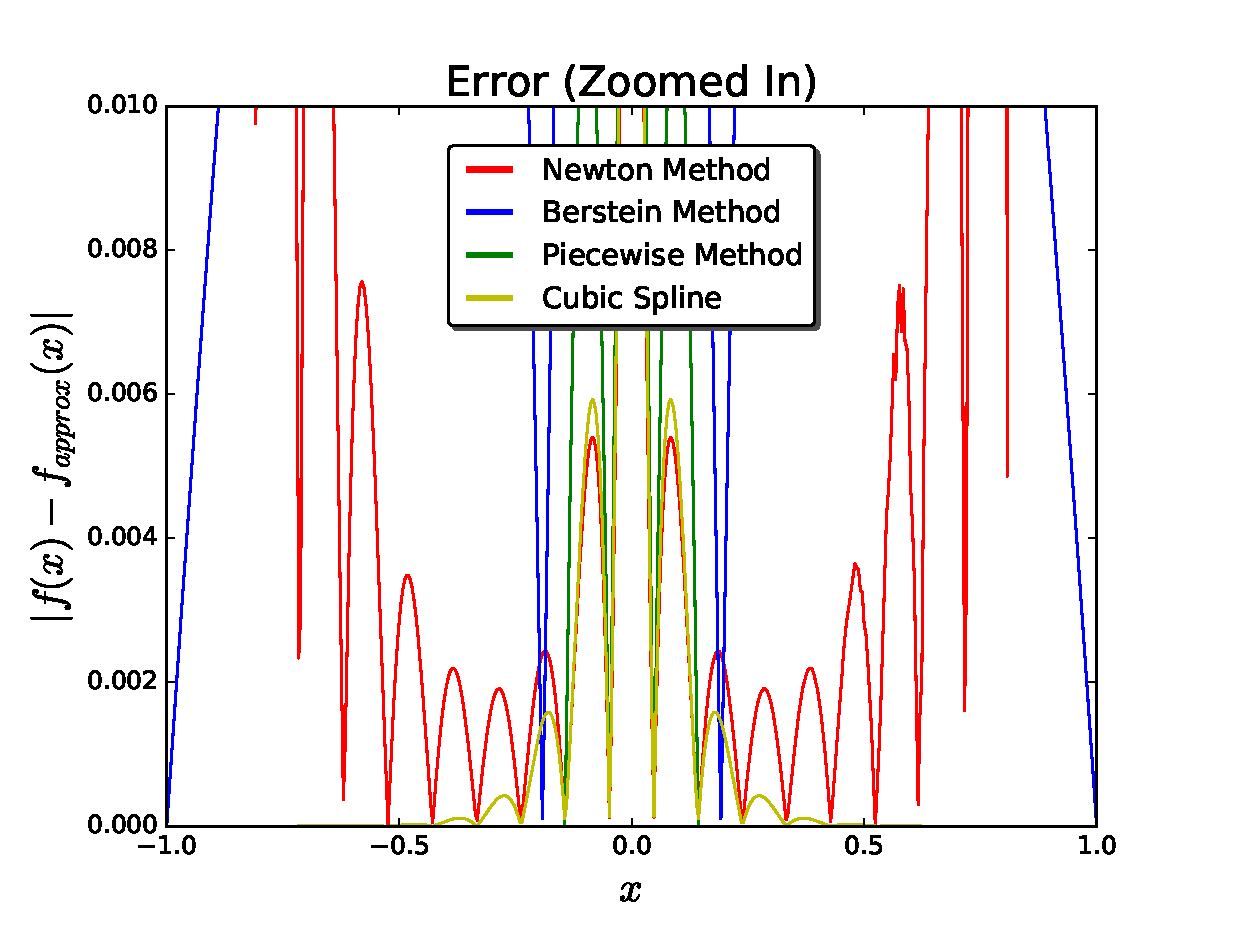
\includegraphics[width=1.1\linewidth]{errorFigg3.eps}
		\caption{Local view of error.}
		\label{fig:sub2}
	\end{subfigure}
	\caption{Error for interpolating methods $f_{approx}(x)$ vs exact $f(x) = \vert x \vert + x/2 - x^2$ (double precision evaluation). }
	\label{fig:test}
\end{figure}

\begin{figure}[H]
	\centering
	\begin{subfigure}{.5\textwidth}
		\centering
		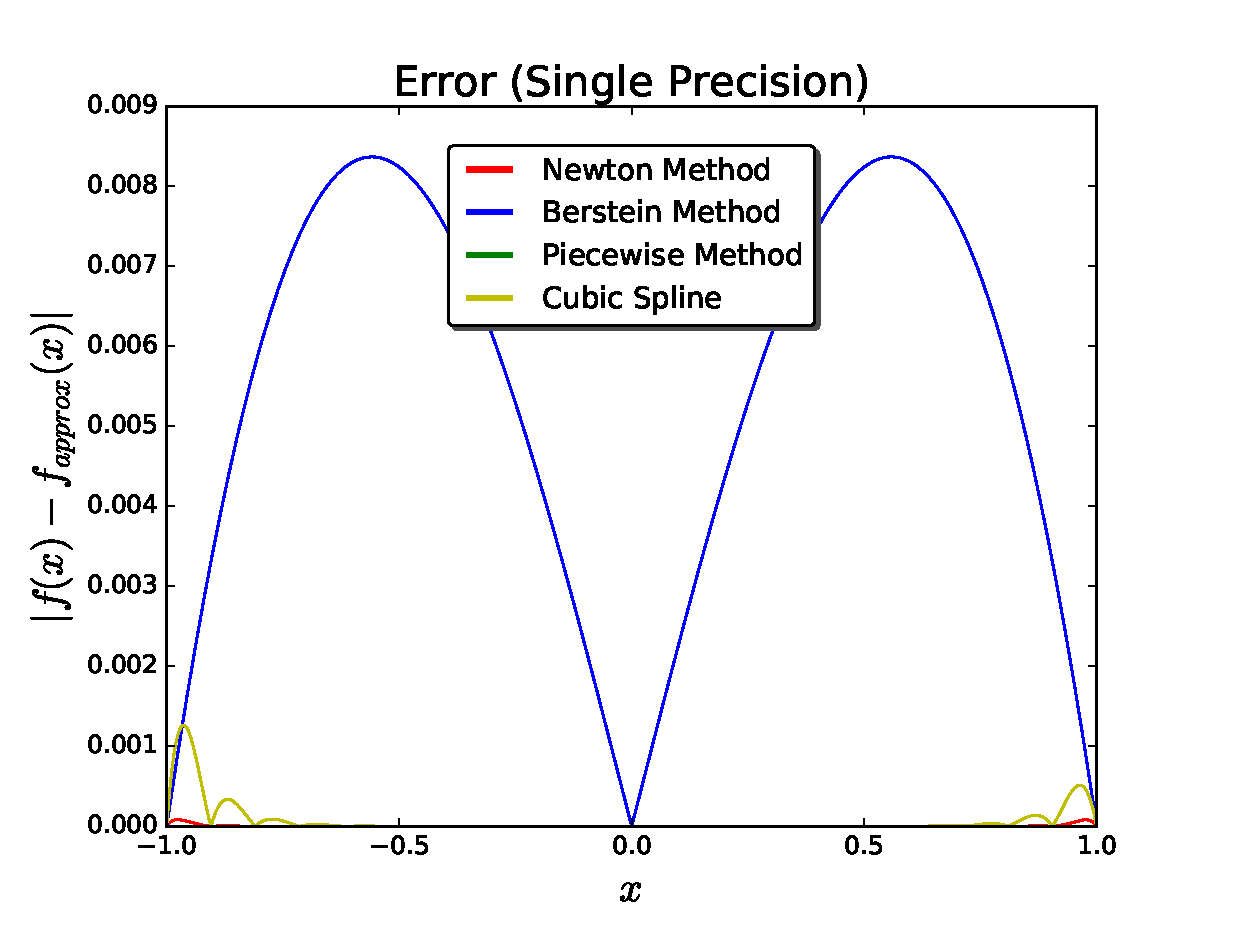
\includegraphics[width=1.1\linewidth]{errorFig4.eps}
		\caption{Global view of error.}
		\label{fig:sub1}
	\end{subfigure}%
	\begin{subfigure}{.5\textwidth}
		\centering
		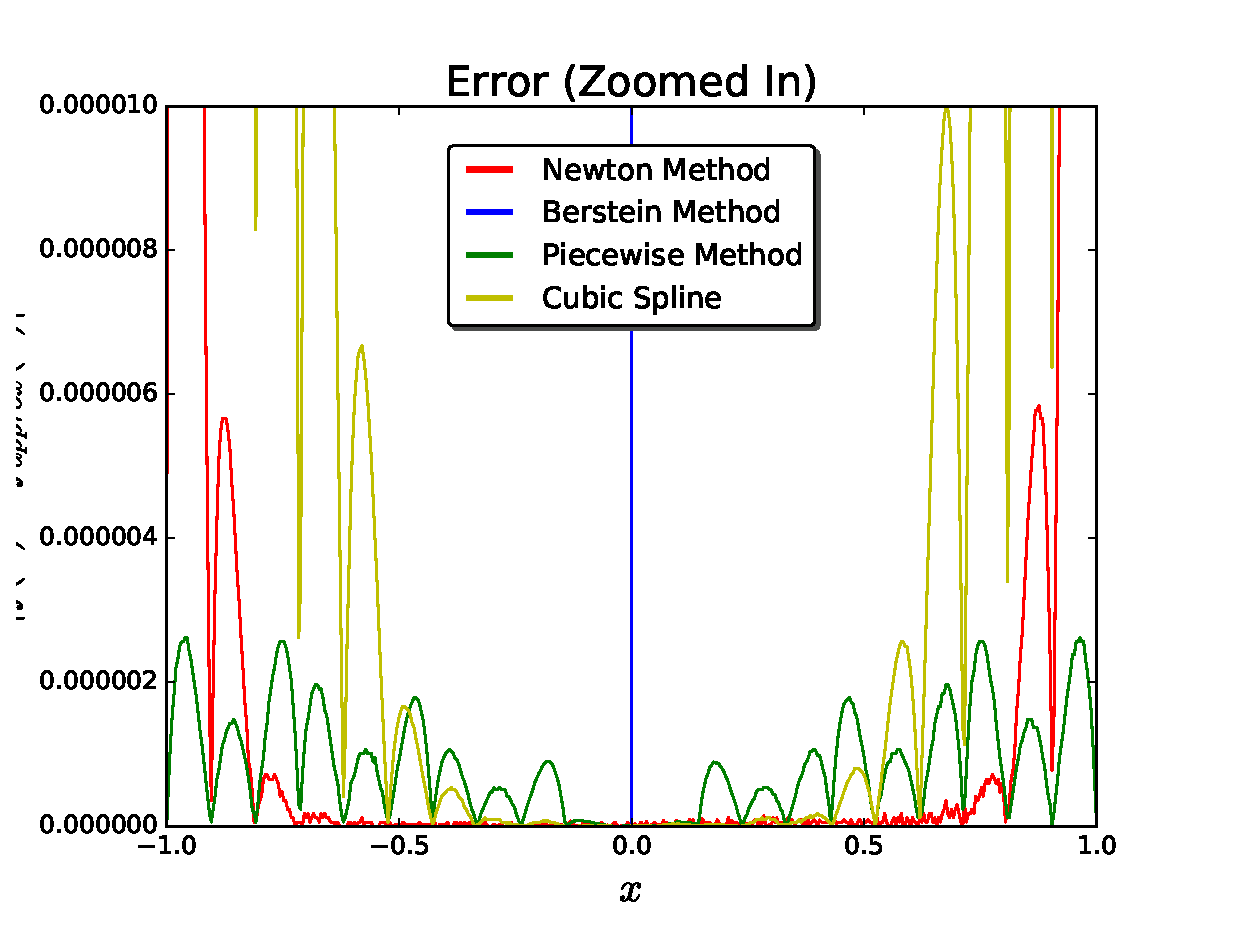
\includegraphics[width=1.1\linewidth]{errorFigg4.eps}
		\caption{Local view of error.}
		\label{fig:sub2}
	\end{subfigure}
	\caption{Error for interpolating methods $f_{approx}(x)$ vs exact $f(x) = sin(x)$ (double precision evaluation). }
	\label{fig:test}
\end{figure}

\subsection{Natural Boundary Conditions}

\begin{figure}[H]
	\centering
	\begin{subfigure}{.5\textwidth}
		\centering
		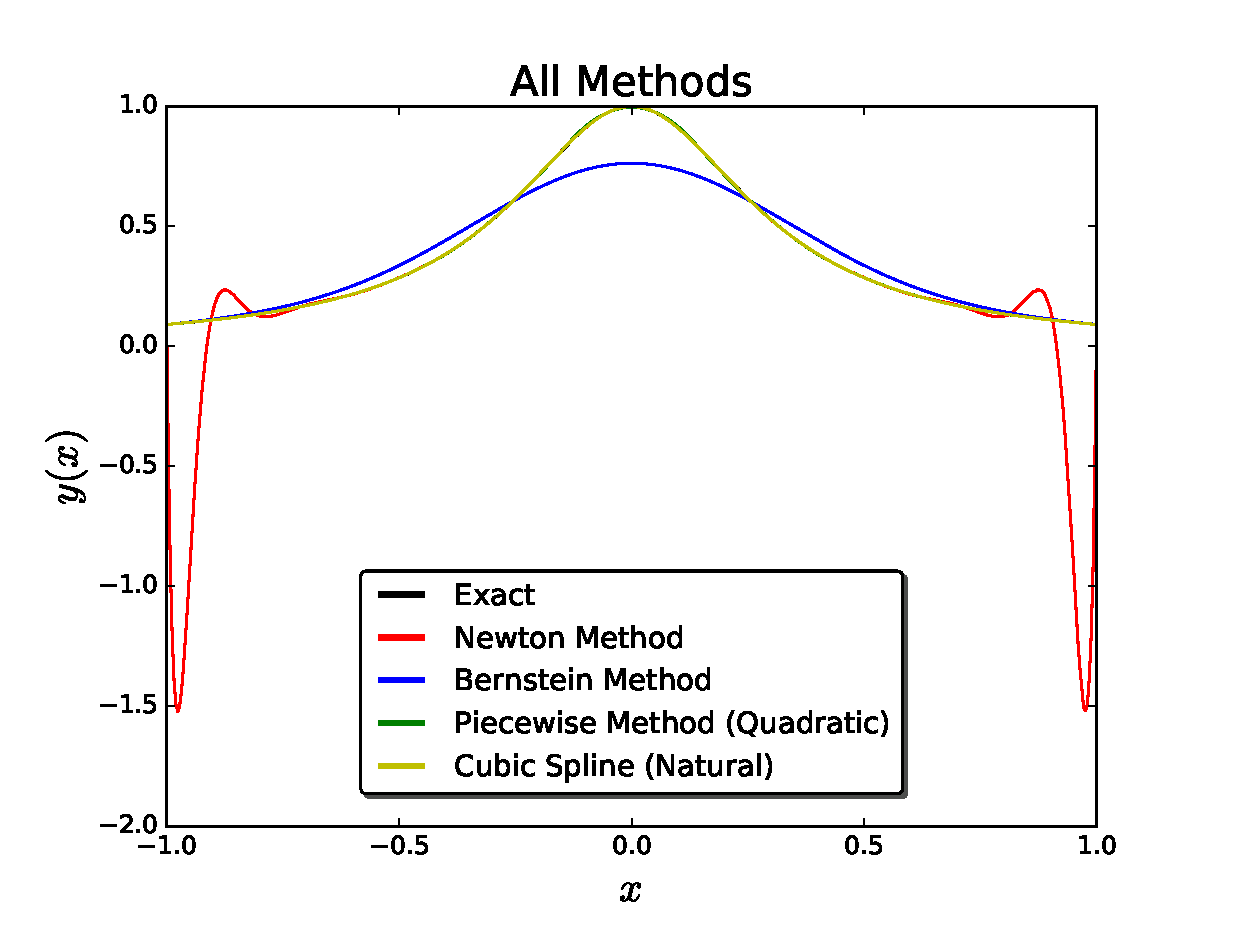
\includegraphics[width=1.1\linewidth]{Nfig1.eps}
		\caption{Global view of error.}
		\label{fig:sub1}
	\end{subfigure}%
	\begin{subfigure}{.5\textwidth}
		\centering
		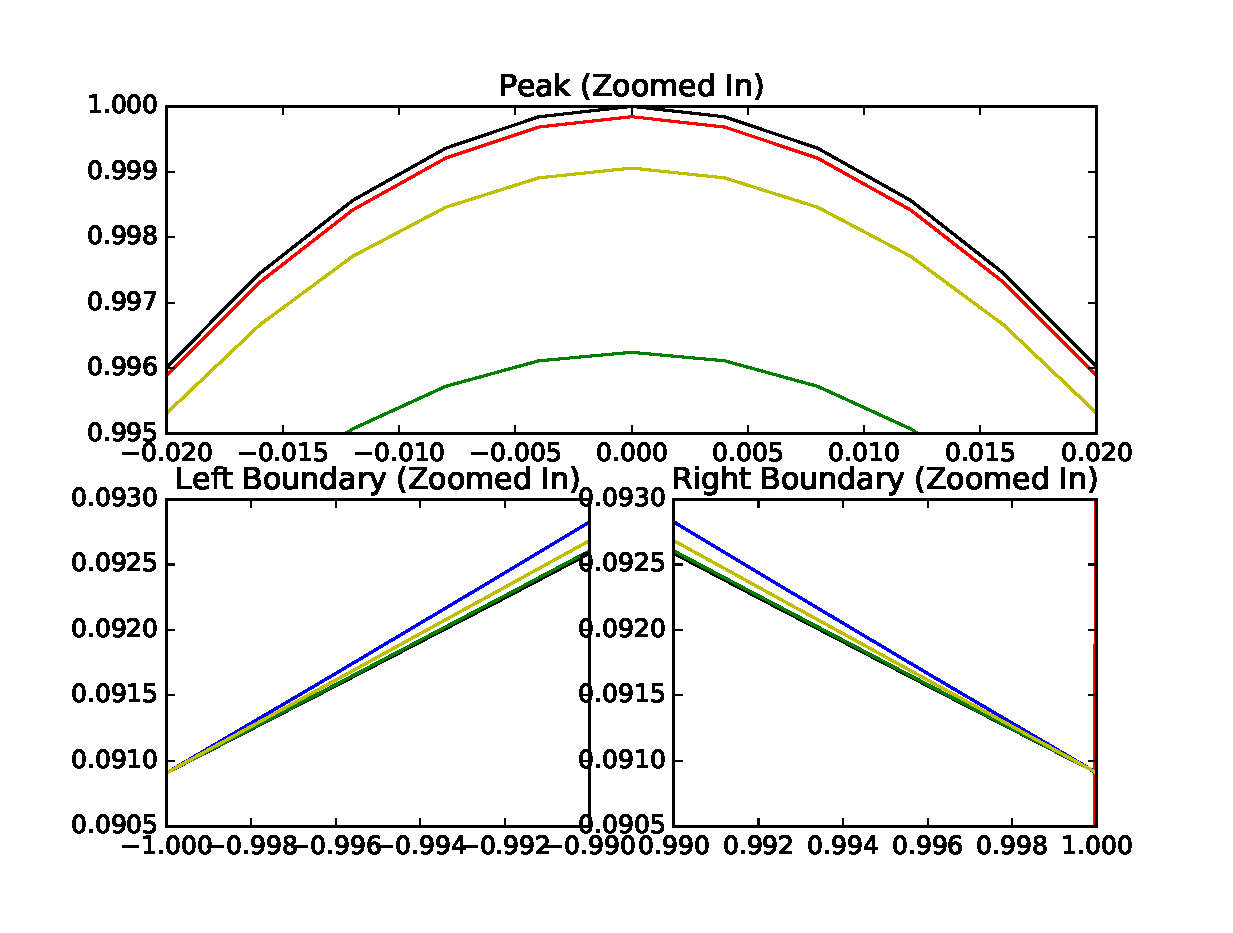
\includegraphics[width=1.1\linewidth]{NsubFig1.eps}
		\caption{Local view of error.}
		\label{fig:sub2}
	\end{subfigure}
	\caption{Error for interpolating methods $f_{approx}(x)$ vs exact $f(x) = 1/(1 + 10x^2)$ (double precision evaluation). }
	\label{fig:test}
\end{figure}

\begin{figure}[H]
	\centering
	\begin{subfigure}{.5\textwidth}
		\centering
		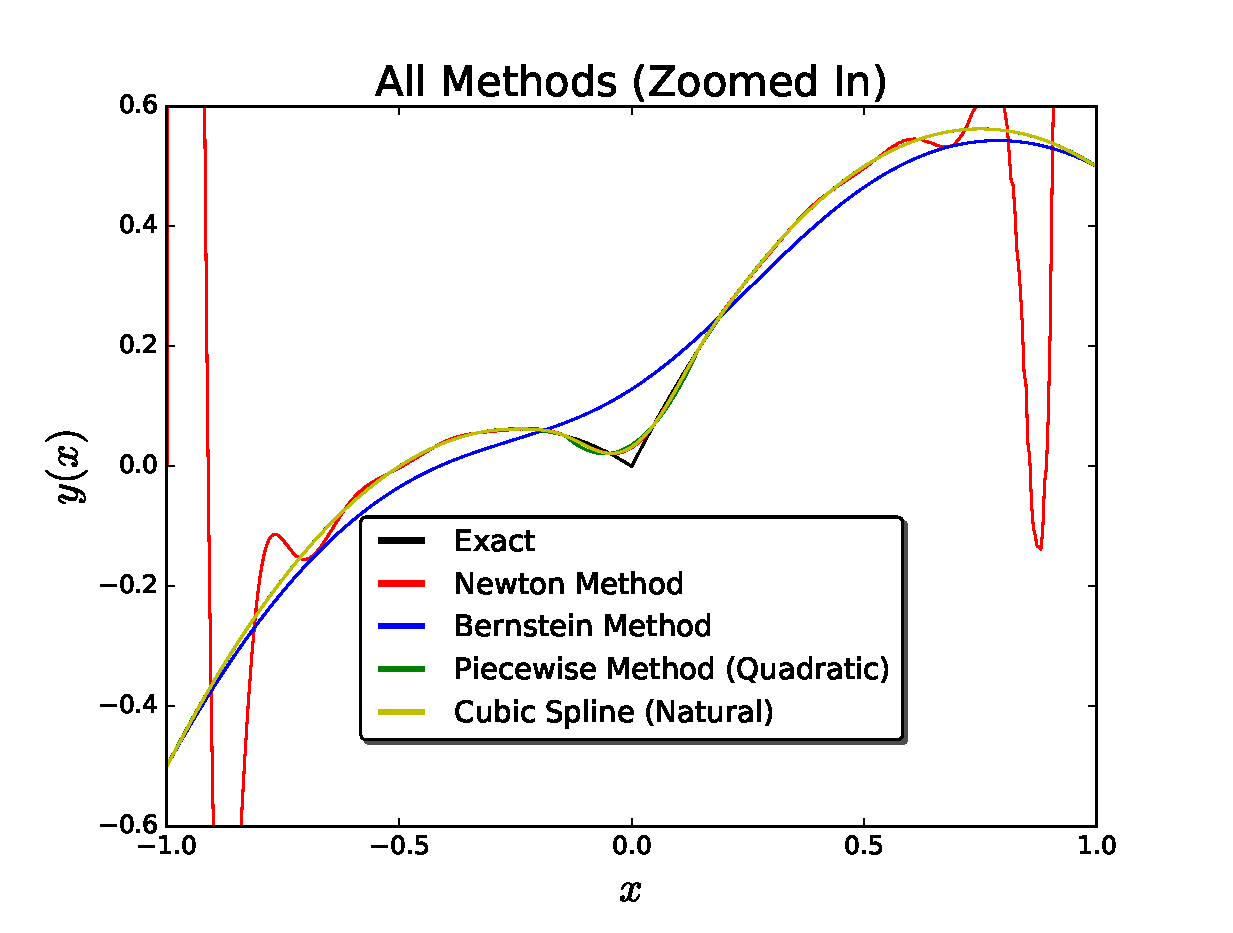
\includegraphics[width=1.1\linewidth]{Nfig3.eps}
		\caption{Global view of error.}
		\label{fig:sub1}
	\end{subfigure}%
	\begin{subfigure}{.5\textwidth}
		\centering
		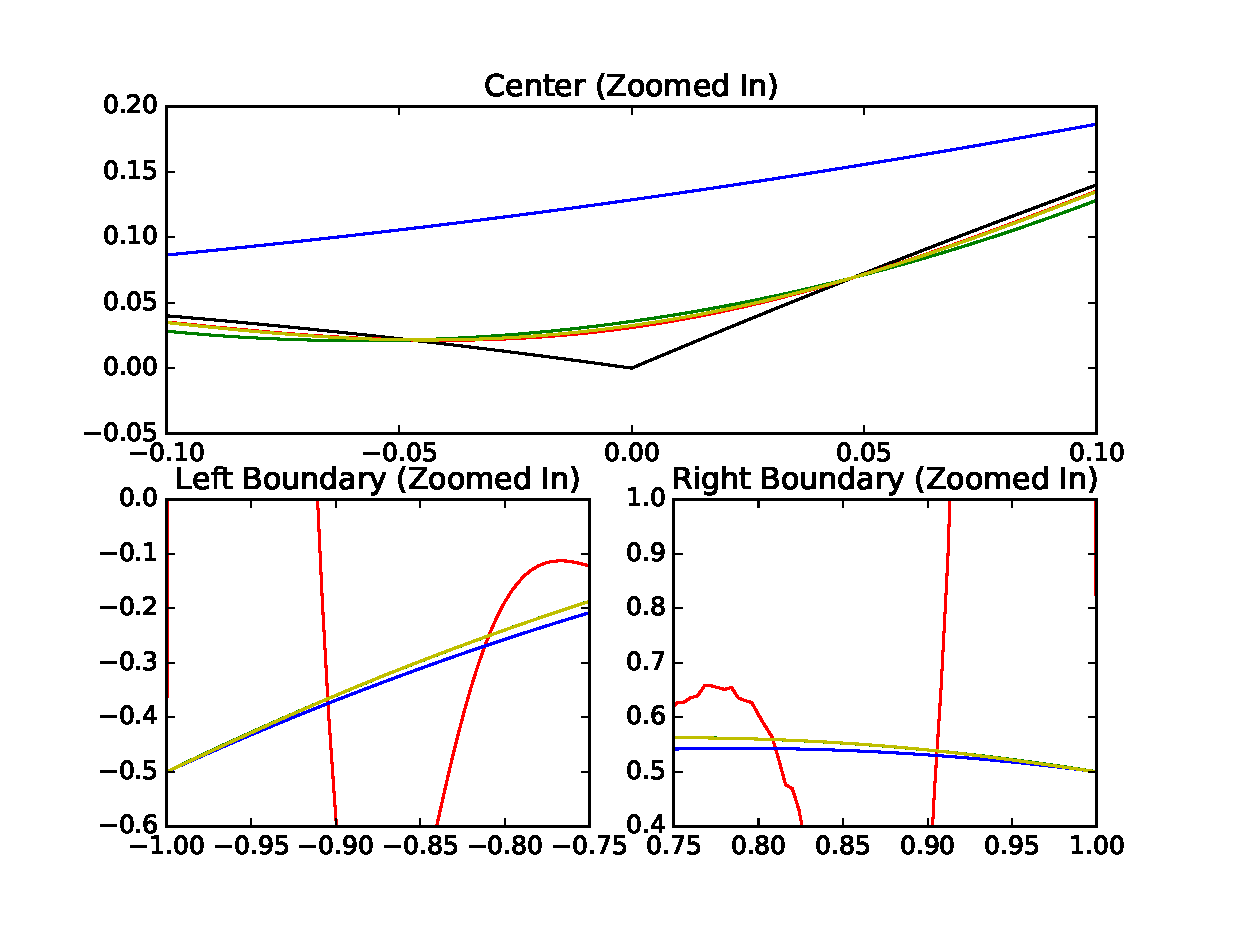
\includegraphics[width=1.1\linewidth]{NsubFig3.eps}
		\caption{Local view of error.}
		\label{fig:sub2}
	\end{subfigure}
	\caption{Error for interpolating methods $f_{approx}(x)$ vs exact $f(x) = \vert x \vert + x/2 - x^2$ (double precision evaluation). }
	\label{fig:test}
\end{figure}

\begin{figure}[H]
	\centering
	\begin{subfigure}{.5\textwidth}
		\centering
		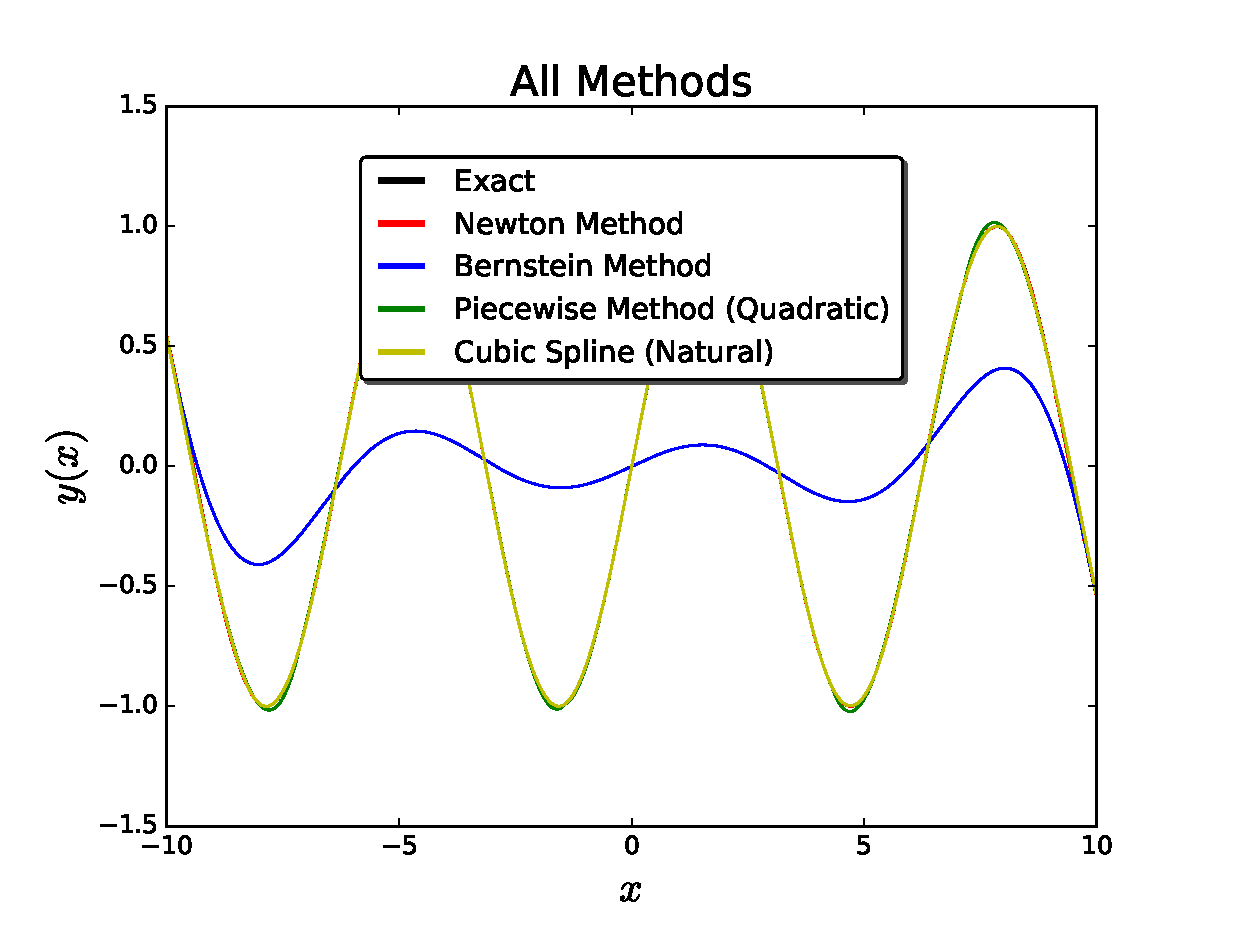
\includegraphics[width=1.1\linewidth]{Nfig4.eps}
		\caption{Global view of error.}
		\label{fig:sub1}
	\end{subfigure}%
	\begin{subfigure}{.5\textwidth}
		\centering
		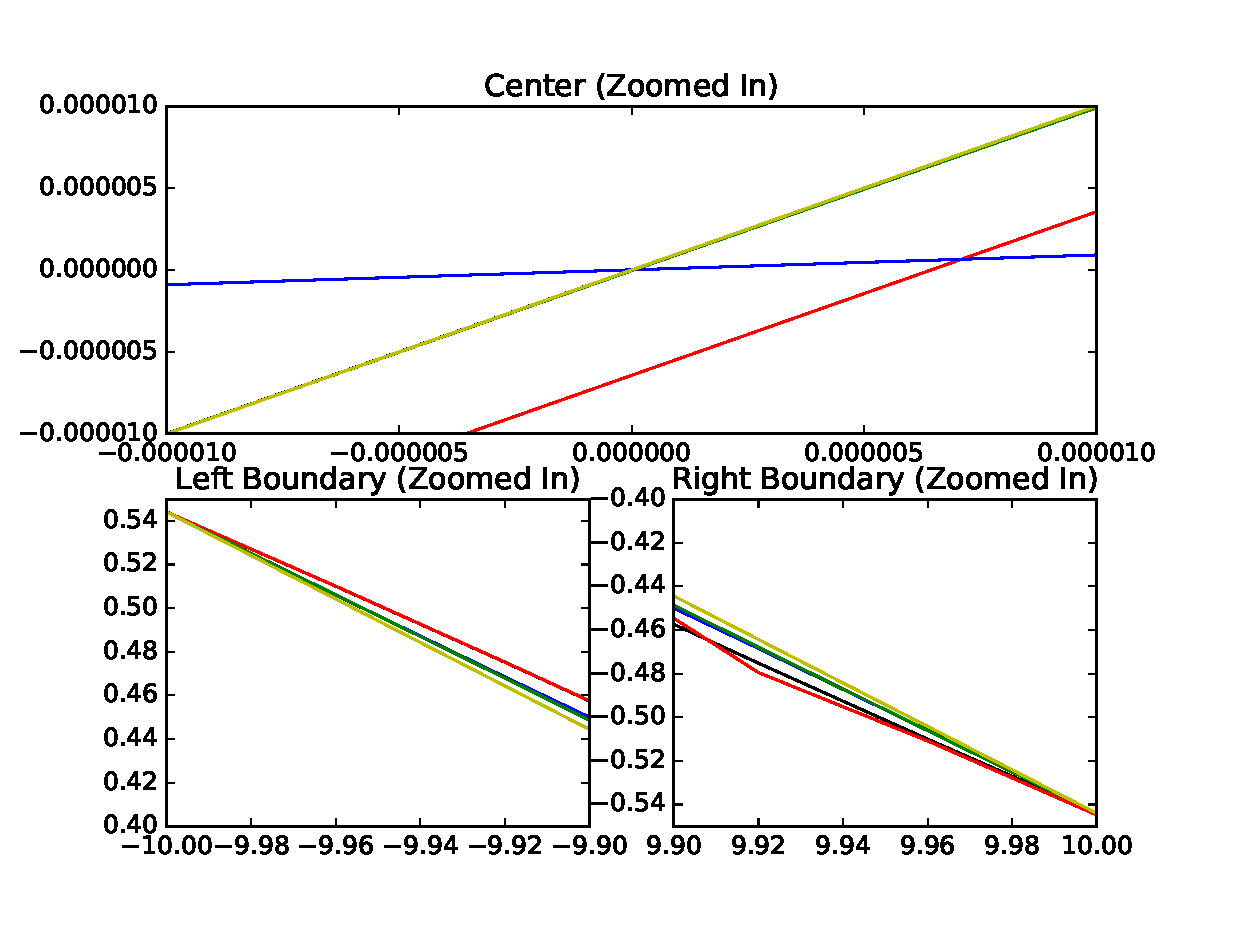
\includegraphics[width=1.1\linewidth]{NsubFig4.eps}
		\caption{Local view of error.}
		\label{fig:sub2}
	\end{subfigure}
	\caption{Error for interpolating methods $f_{approx}(x)$ vs exact $f(x) = sin(x)$ (double precision evaluation). }
	\label{fig:test}
\end{figure}

\begin{figure}[H]
	\centering
	\begin{subfigure}{.5\textwidth}
		\centering
		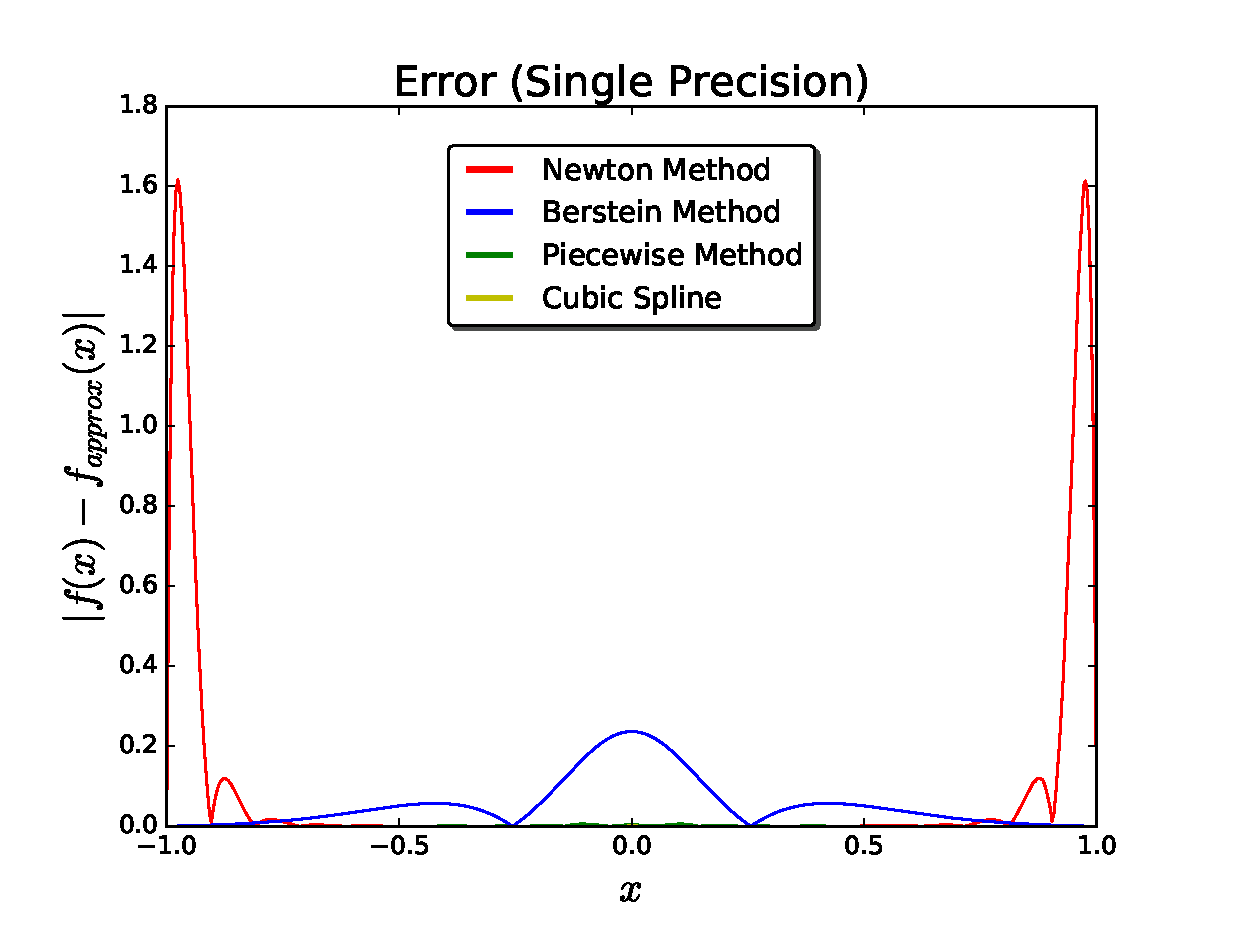
\includegraphics[width=1.1\linewidth]{NerrorFig1.eps}
		\caption{Global view of error.}
		\label{fig:sub1}
	\end{subfigure}%
	\begin{subfigure}{.5\textwidth}
		\centering
		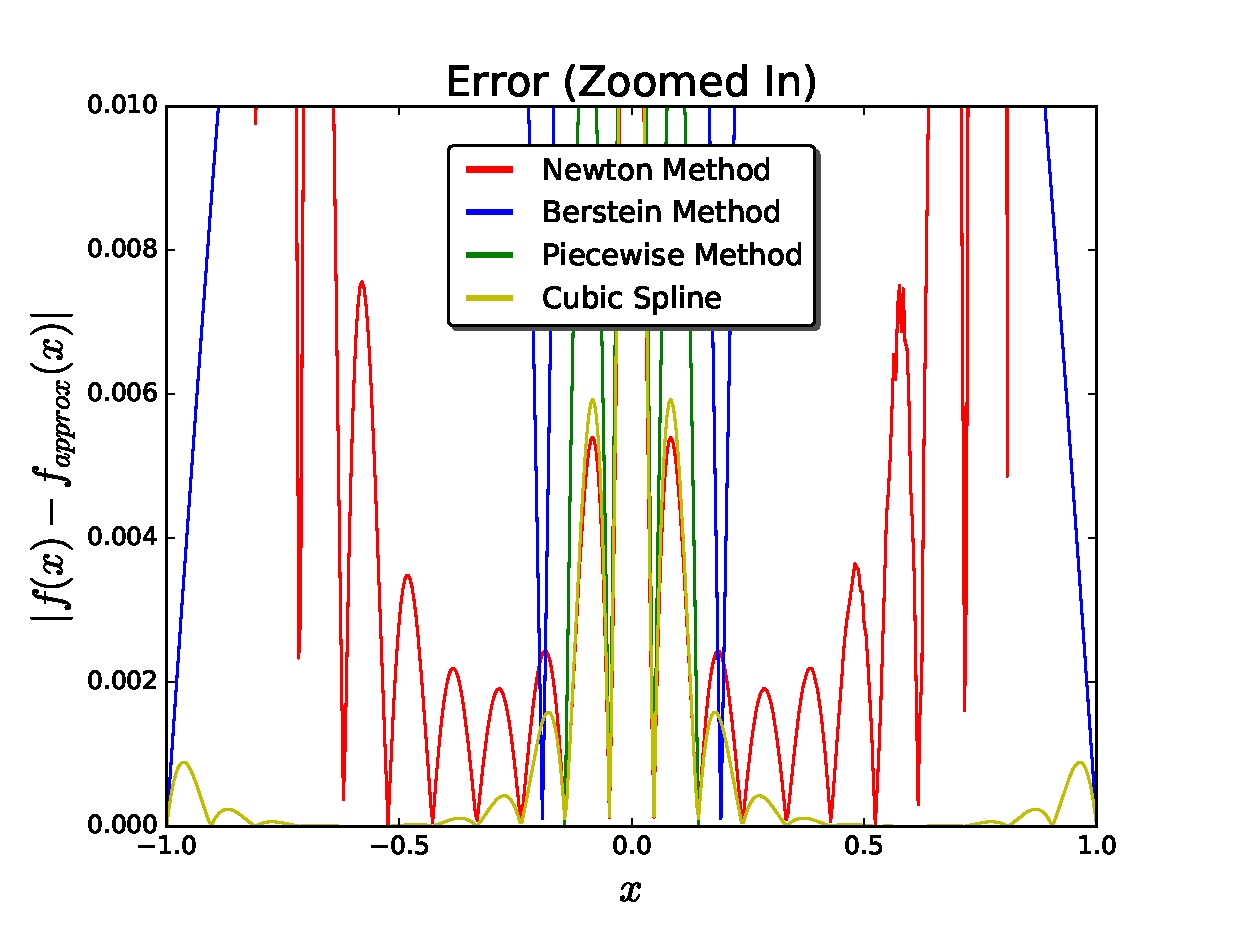
\includegraphics[width=1.1\linewidth]{NerrorFigg1.eps}
		\caption{Local view of error.}
		\label{fig:sub2}
	\end{subfigure}
	\caption{Error for interpolating methods $f_{approx}(x)$ vs exact $f(x) = 1/(1 + 10x^2)$ (double precision evaluation). }
	\label{fig:test}
\end{figure}

\begin{figure}[H]
	\centering
	\begin{subfigure}{.5\textwidth}
		\centering
		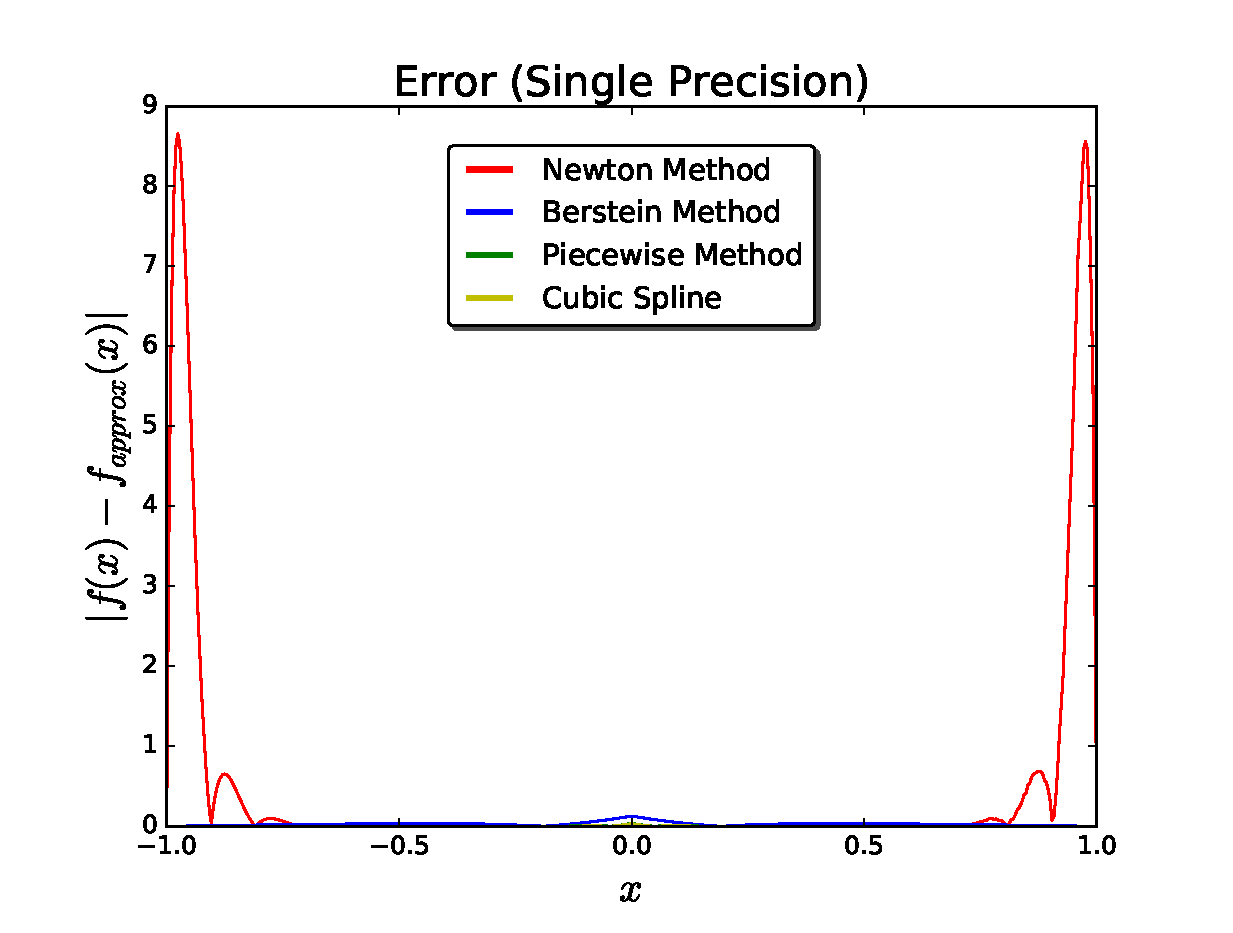
\includegraphics[width=1.1\linewidth]{NerrorFig3.eps}
		\caption{Global view of error.}
		\label{fig:sub1}
	\end{subfigure}%
	\begin{subfigure}{.5\textwidth}
		\centering
		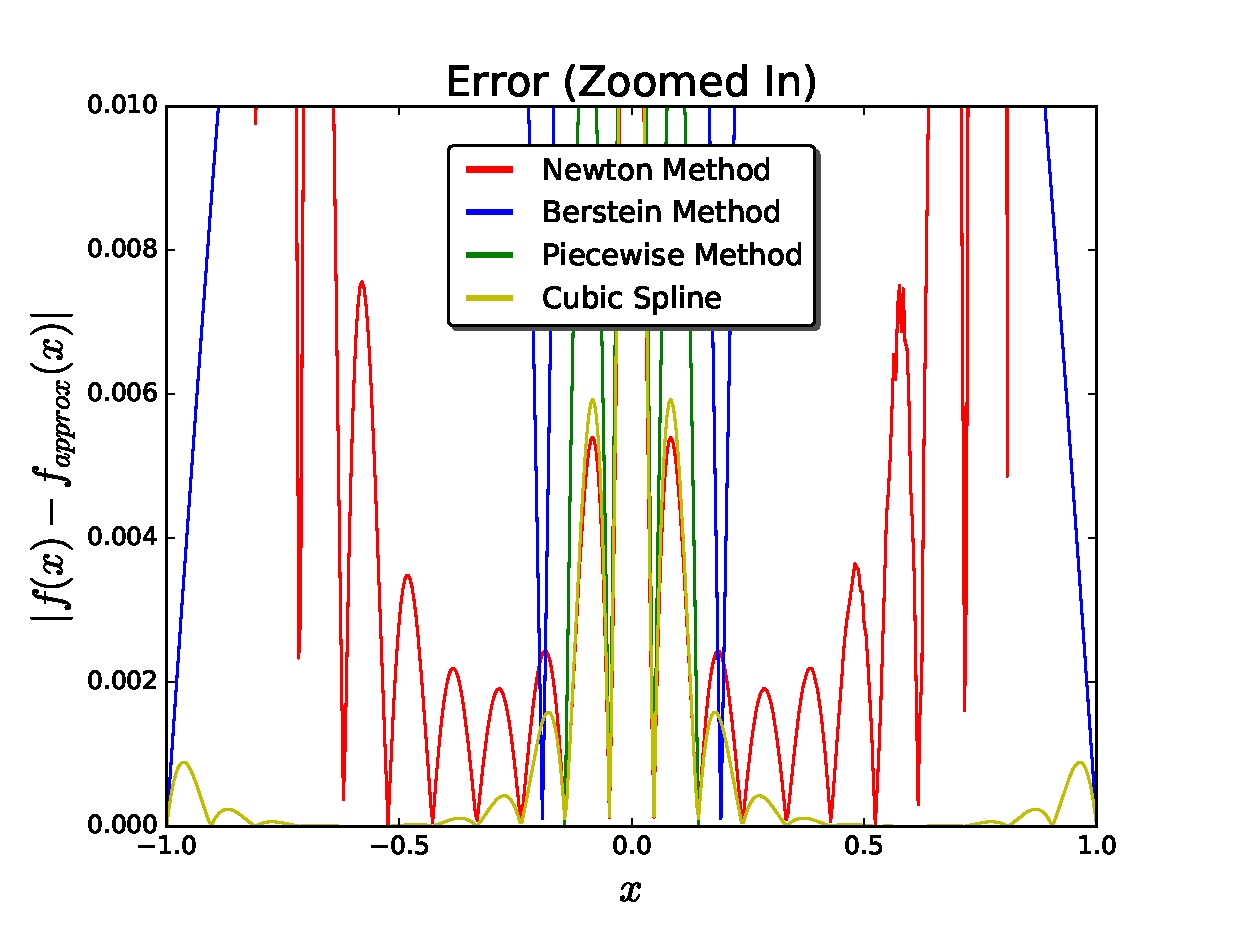
\includegraphics[width=1.1\linewidth]{NerrorFigg3.eps}
		\caption{Local view of error.}
		\label{fig:sub2}
	\end{subfigure}
	\caption{Error for interpolating methods $f_{approx}(x)$ vs exact $f(x) = \vert x \vert + x/2 - x^2$ (double precision evaluation). }
	\label{fig:test}
\end{figure}

\begin{figure}[H]
	\centering
	\begin{subfigure}{.5\textwidth}
		\centering
		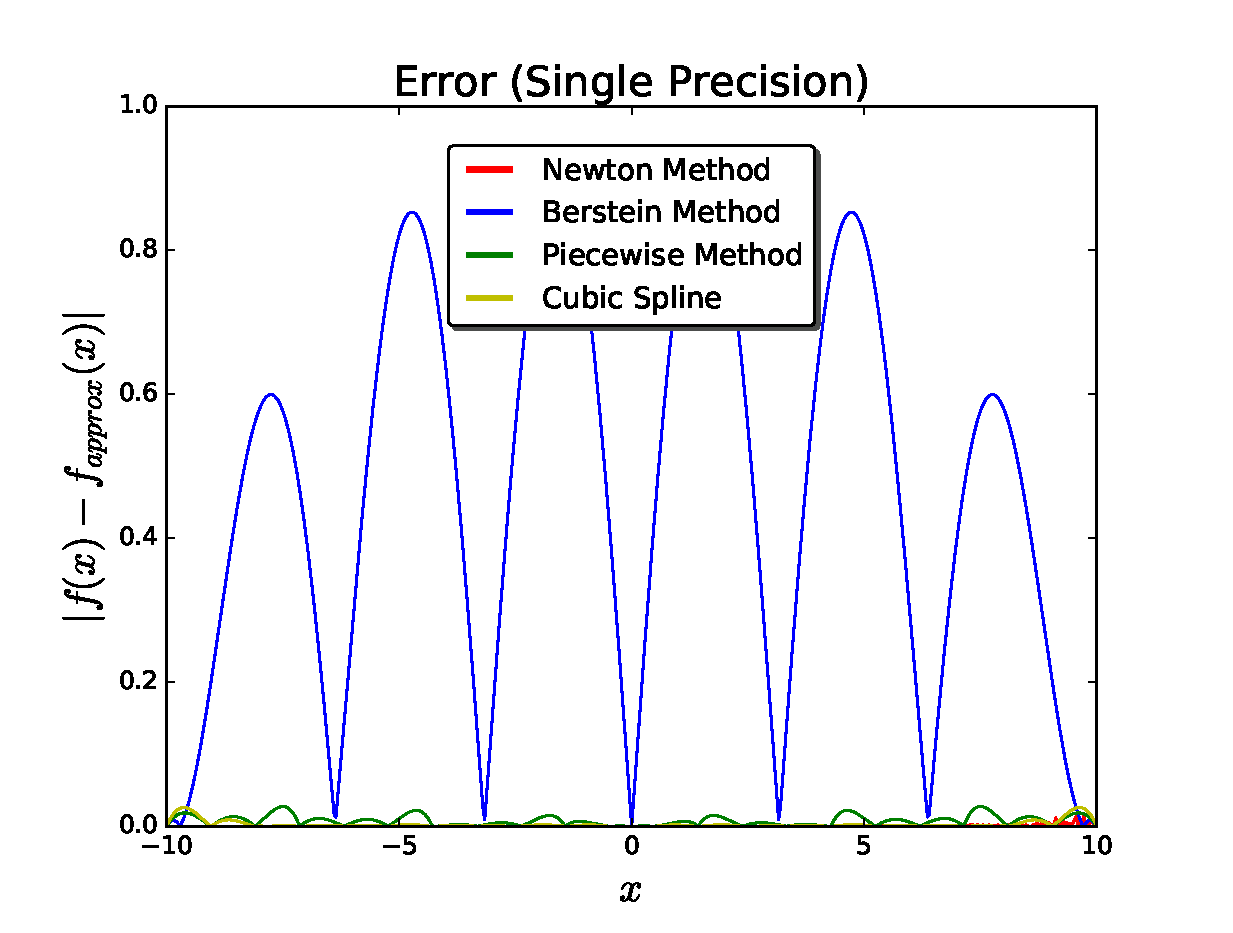
\includegraphics[width=1.1\linewidth]{NerrorFig4.eps}
		\caption{Global view of error.}
		\label{fig:sub1}
	\end{subfigure}%
	\begin{subfigure}{.5\textwidth}
		\centering
		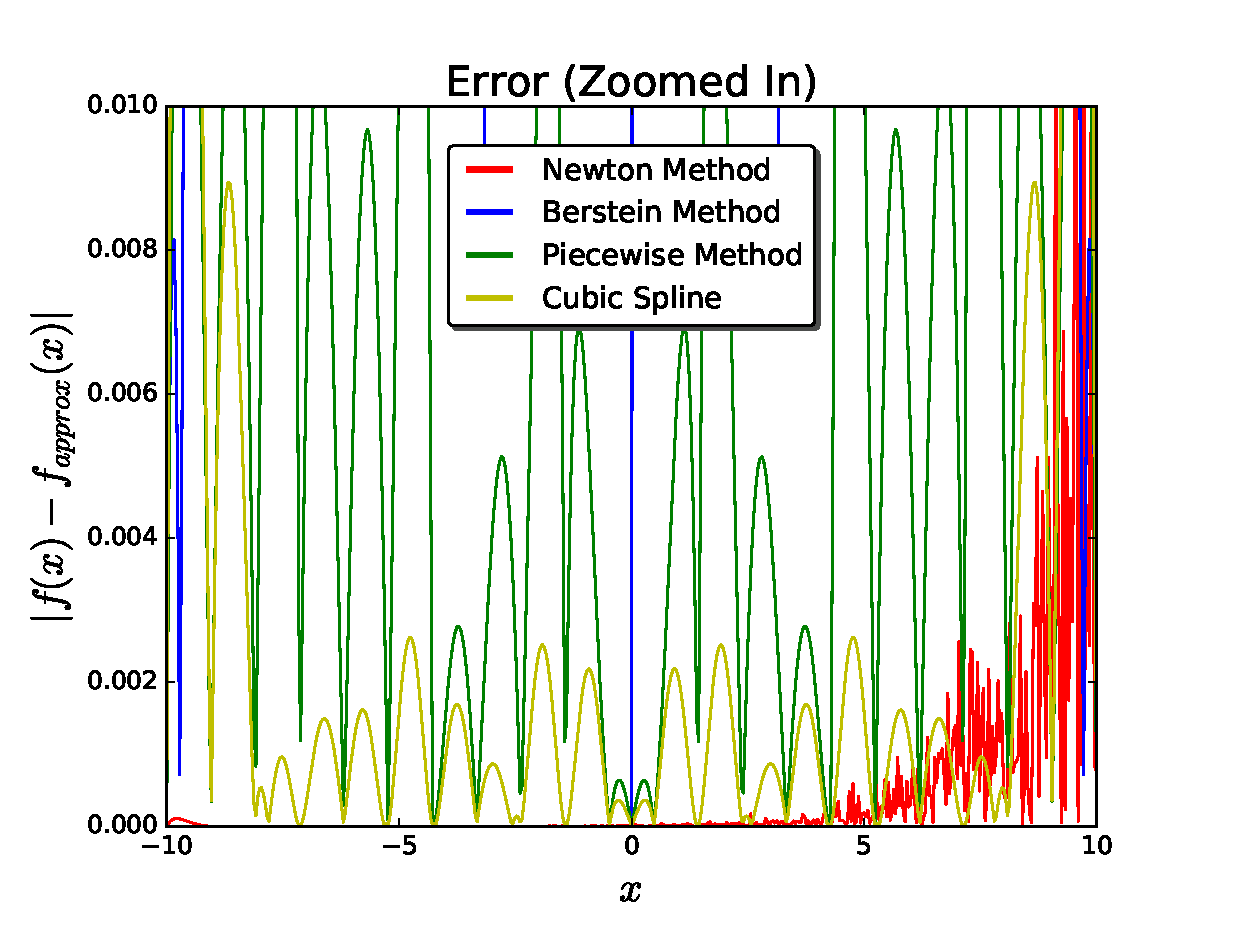
\includegraphics[width=1.1\linewidth]{NerrorFigg4.eps}
		\caption{Local view of error.}
		\label{fig:sub2}
	\end{subfigure}
	\caption{Error for interpolating methods $f_{approx}(x)$ vs exact $f(x) = sin(x)$ (double precision evaluation). }
	\label{fig:test}
\end{figure}

\subsection{Other Figures}

\begin{figure}[H]
	\centering
	\begin{subfigure}{.5\textwidth}
		\centering
		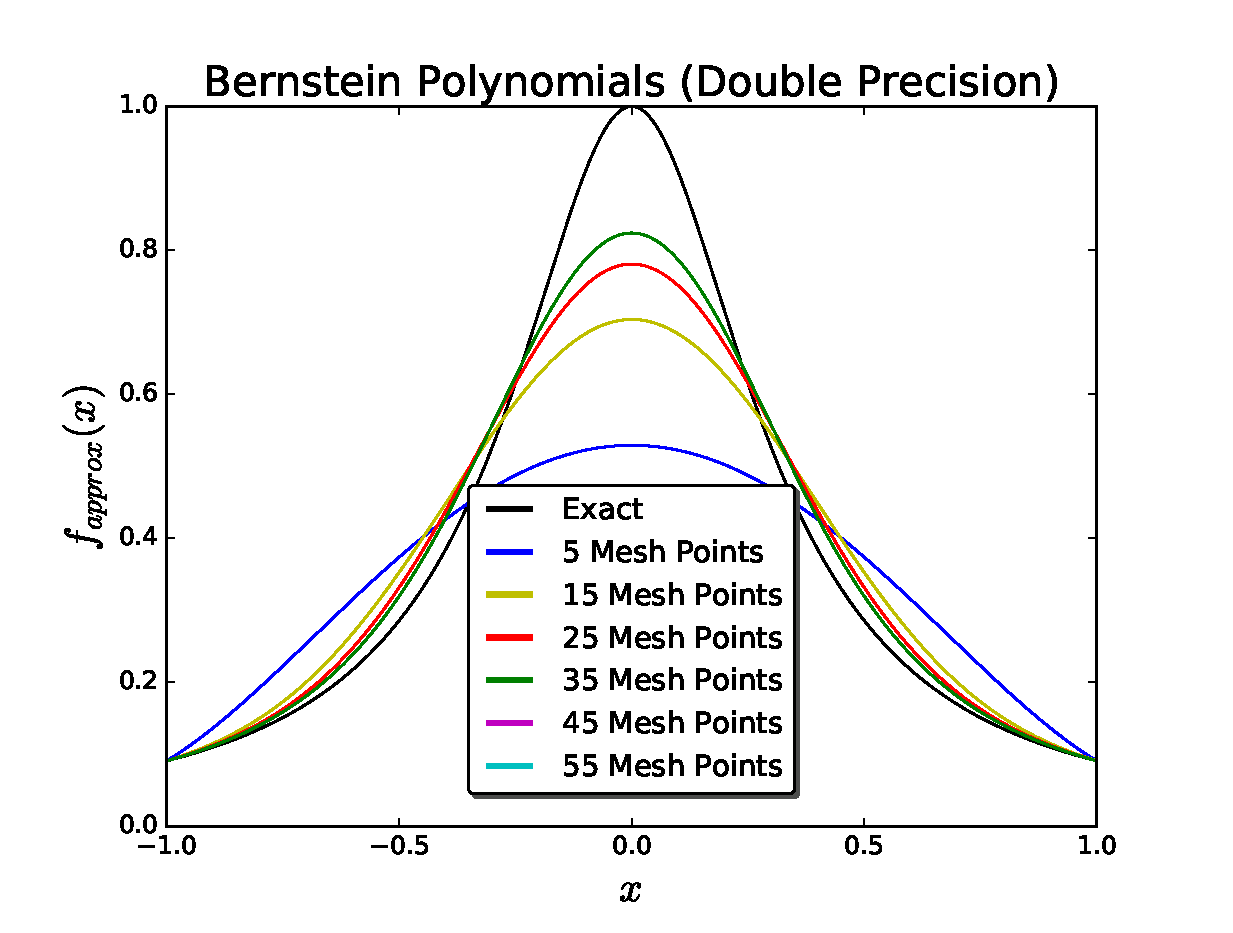
\includegraphics[width=1.1\linewidth]{bernSingle.eps}
		\caption{Single Precision.}
		\label{fig:sub1}
	\end{subfigure}%
	\begin{subfigure}{.5\textwidth}
		\centering
		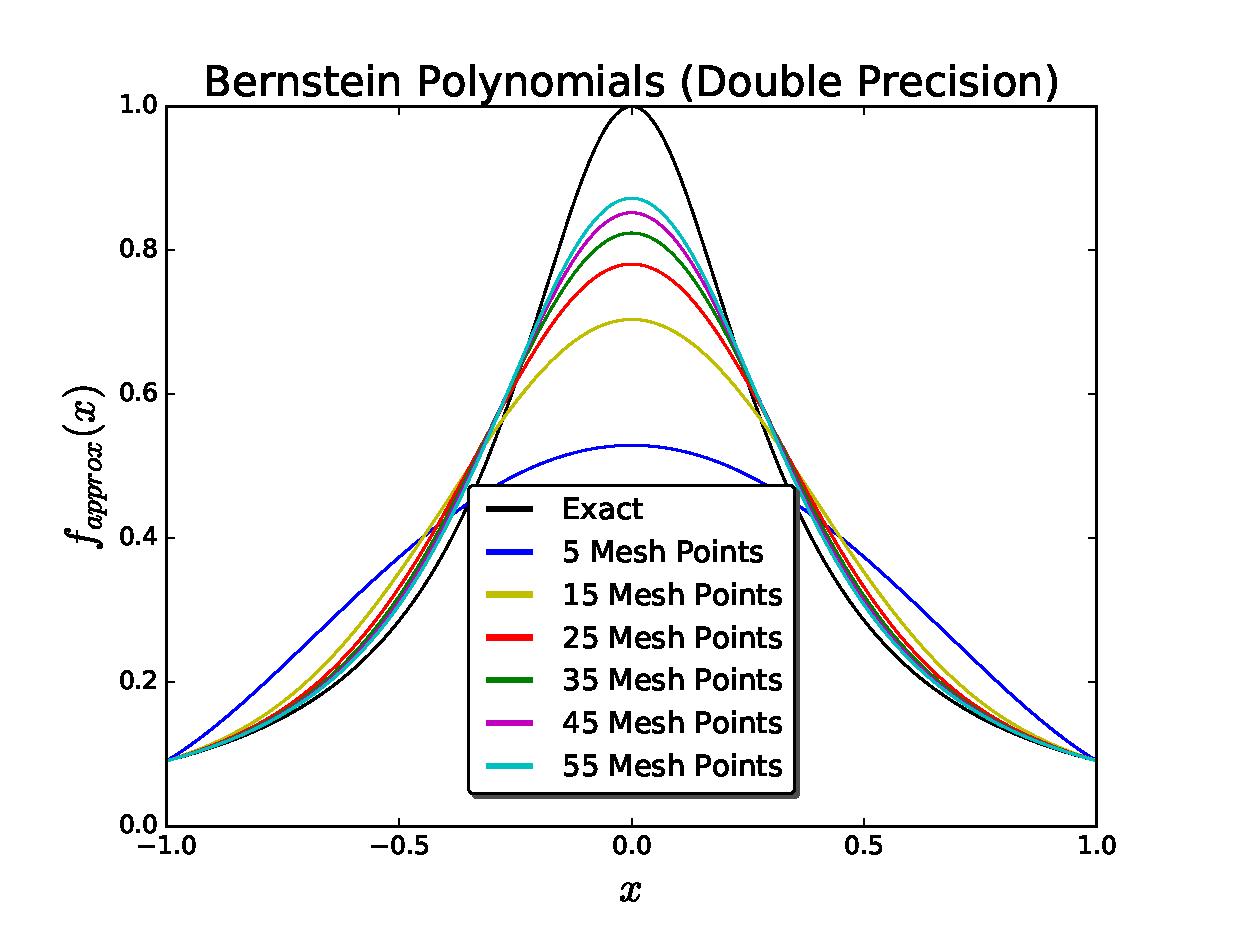
\includegraphics[width=1.1\linewidth]{bernDouble.eps}
		\caption{Double precision.}
		\label{fig:sub2}
	\end{subfigure}
	\caption{Bernstein polynomials converge to our function but can only do as well as the precision set.}
	\label{fig:test}
\end{figure}

\end{document}
